\chapter{Měření hysterezních smyček}
V této kapitole se věnujeme studiu hysterezních smyček. 
Studujeme pouze tzv. majoritní hysterezní smyčky, které začínají a končí v dostatečně vysokých polích (na koncích smyčky je magnetizace ve směru vnějšího pole).
V majoritních hysterezních smyčkách typicky dochází ke dvěma přeskokům magnetizace, při koercitivních polích $\hcj$ a $\hcd$ \cite{Reichlova}.

Měřením Voigtova jevu a MLD u hysterezních smyček určujeme koercitivní pole $\hcj$ a $\hcd$ a amplitudy přeskoku $A$ a $\Delta B$, ze kterých lze případně určit $\pmld$, součin $\pmld \sin(\xi)$ a směry snadných os.


Měření v nekolineární geometrii na stejném vzorku proběhlo už v práci \cite{Reichlova}, a proto stejný experiment použijeme jako první magnetooptické měření s dvoudimenzionálním elektromagnetem k ověření jeho funkčnosti a použitelnosti.

\section{Metoda měření a zpracování dat} \label{zpracovani_smycek}
Hysterezní smyčky měříme vždy při fixované rovině polarizace $\beta$ a směru vnějšího pole $\phH$.
Znaménko $\hext$ volíme tak, aby kladné hodnoty byly ve směru, který uvádíme. První část smyčky (ze záporných $\hext$ do kladných) označujeme jako \emph{up} a druhou část (z kladných do záporných) \emph{down}.
Up a down zpracováváme zcela odděleně a díky symetrii očekáváme stejné výsledky.

Nejprve vyvážíme můstek na jednom okraji hysterezní smyčky a poté při postupné změně $\hext$ měříme rozdílový a součtový signál, ze kterého vypočítáme $\Delta\beta$ podle \eqref{e:mustek}.


Signál $B$ vypočítáme tak, že součtový signál dělíme jeho střední hodnotou během příslušné části hysterezní smyčky a poté odečteme 1 jako v definici \eqref{e:Bdef}.

Způsob, jakým odečítáme hodnoty $A$, $\Delta B$, $\hcj$ a $\hcd$ je znázorněn na obr. \ref{zpracovani}. Význam veličiny $A_r$ je vysvětlen na str. \pageref{e:Ar}.


V textu dále uváděná chyba veličin $A$, $\Delta B$, $\hcj$ a $\hcd$ je odhadnutá maximální chyba, tj. hranice, za kterou už hodnota na první pohled neodpovídá naměřeným datům.

Průběhy veličin $\Delta \beta$ a $B$ v hysterezních smyčkách, které vykreslujeme, jsme pro lepší přehlednost v některých případech posunuli po vertikální ose do jiných hodnot.

\begin{figure}[htbp]\centering
\qq{	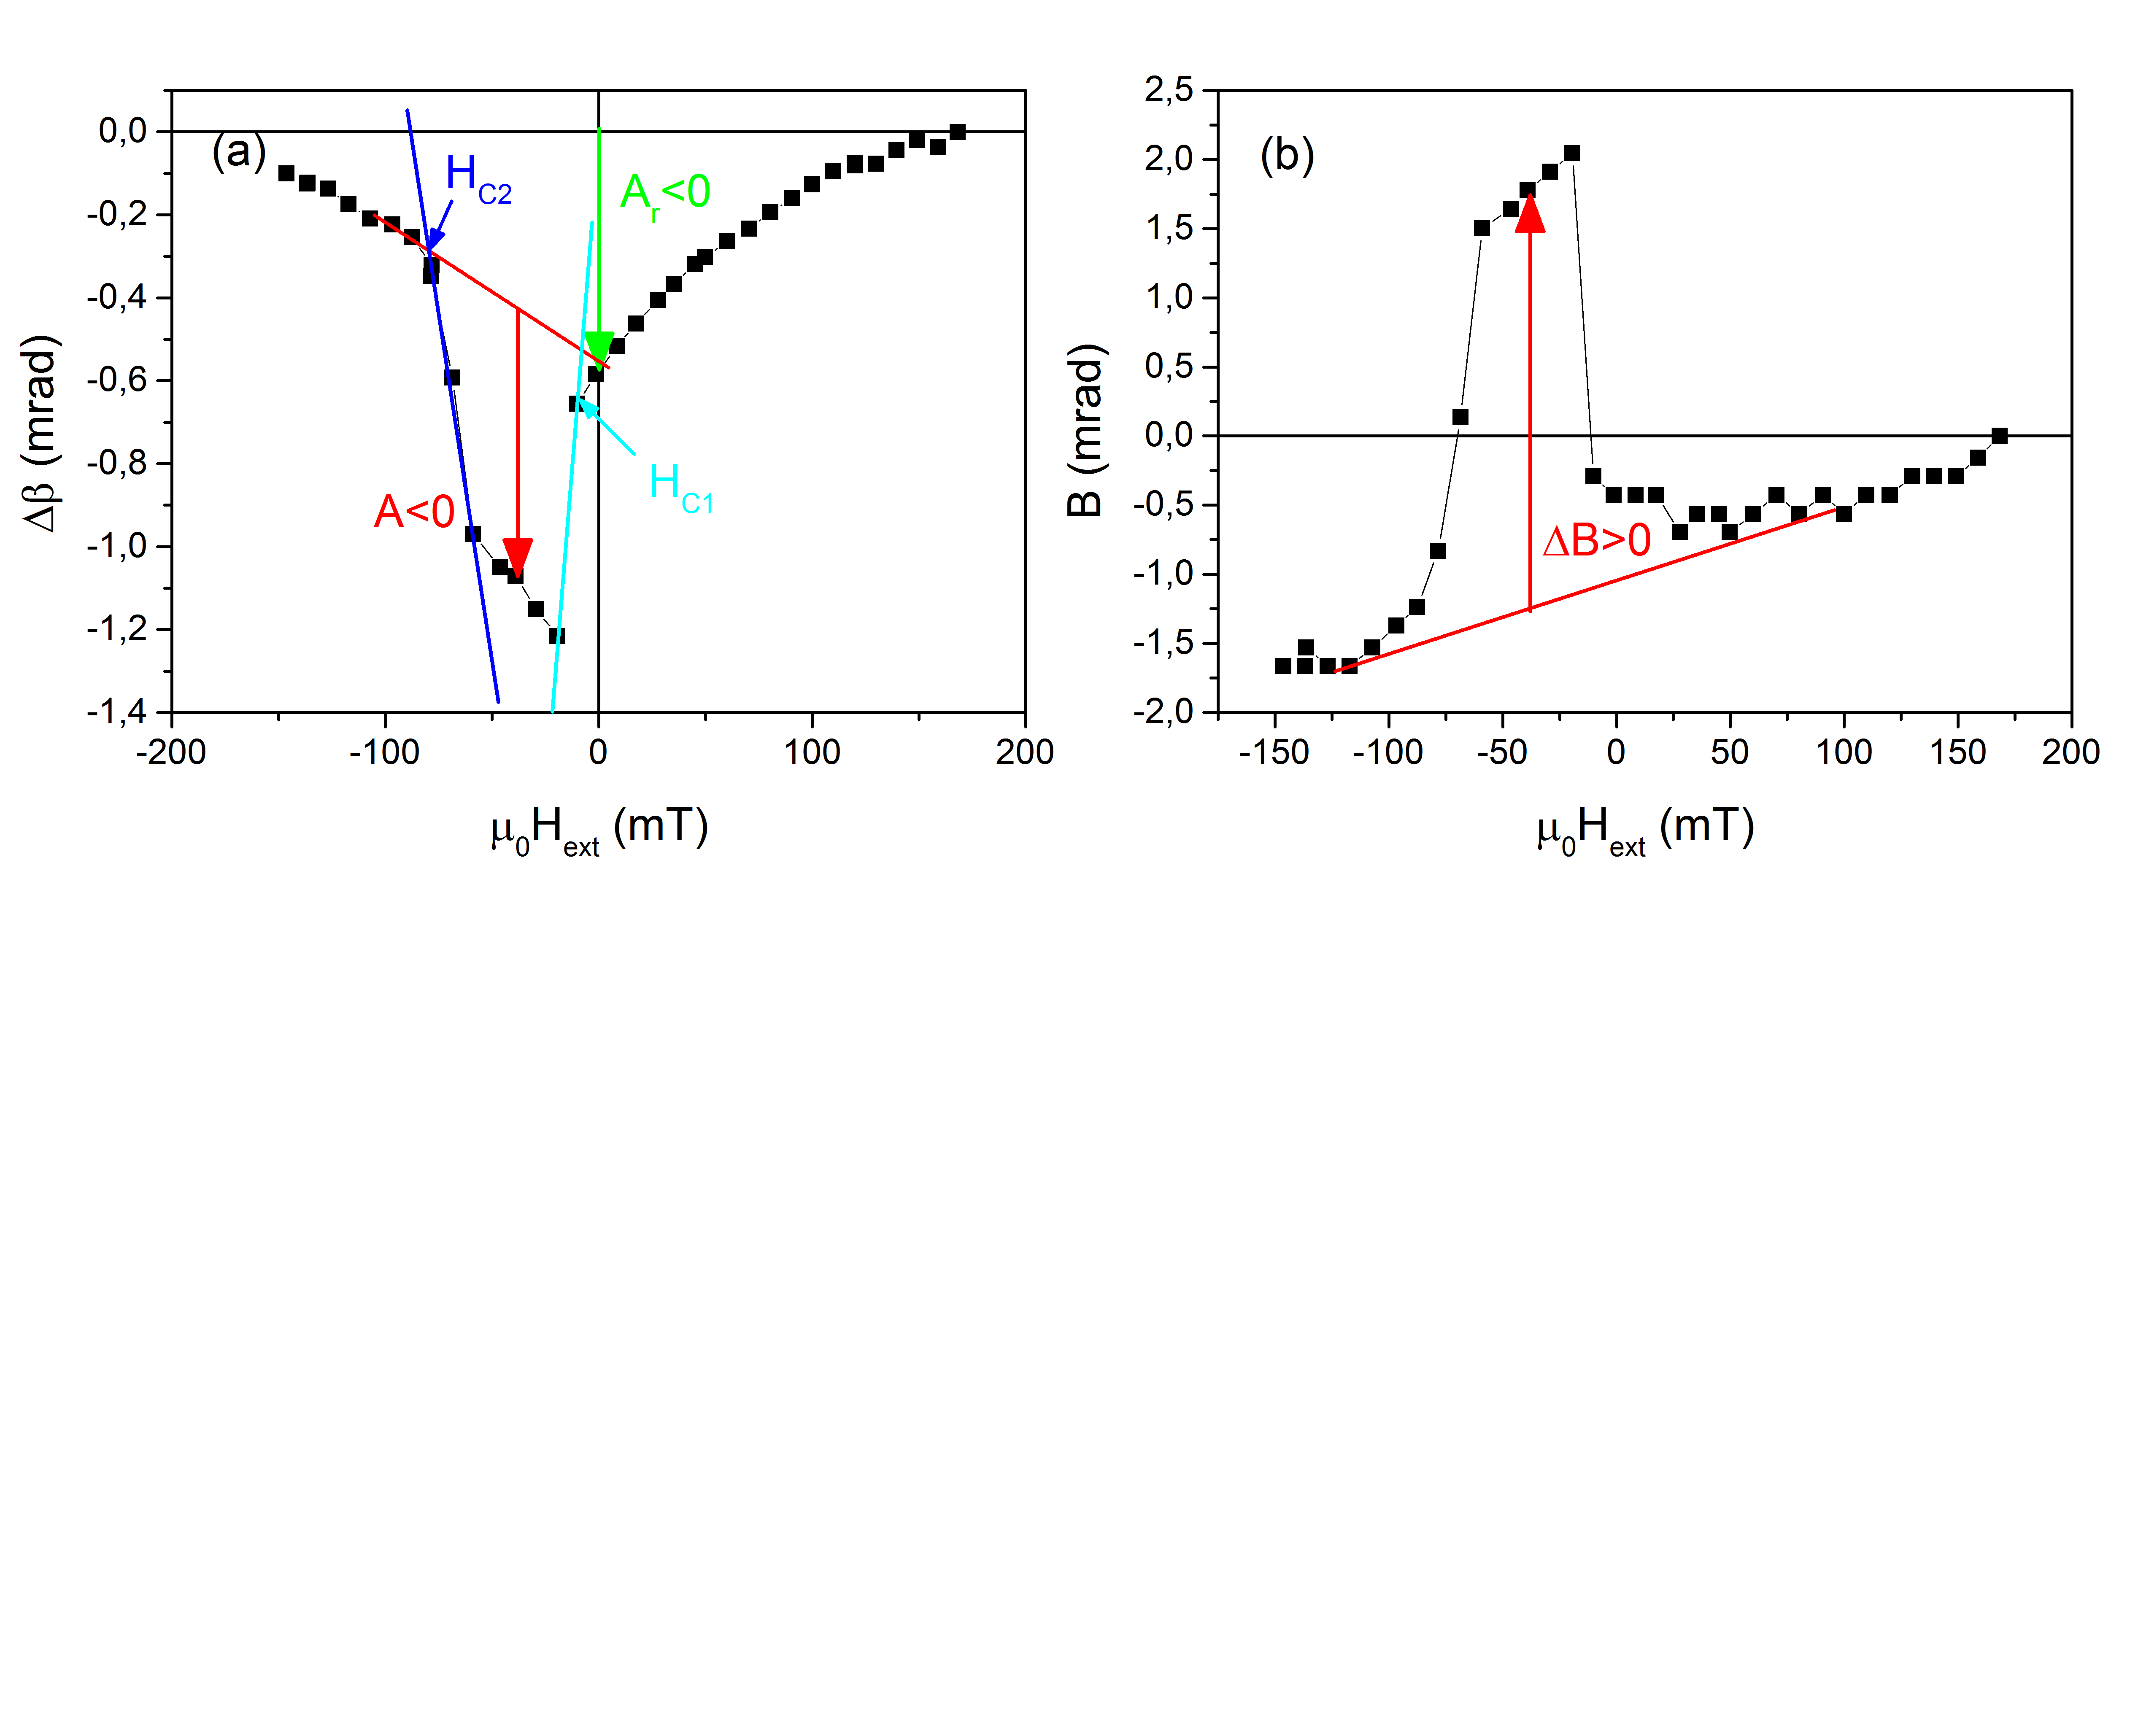
\includegraphics[trim={0 3.43in 0 0}, clip, width=\textwidth]{./png/hyst_zpracovani}}
	\caption{Ilustrace metody určování veličin $A$, $A_r$, $\Delta B$, $\hcj$ a $\hcd$ u hysterezních smyček. Nekolineární geometrie, $\phH=\ang{0}$ pro polarizaci $\beta=\ang{60}$ (a) a $\beta=\ang{30}$ (b).}\label{zpracovani}
\end{figure}

\FloatBarrier


\section{Nekolineární geometrie}
Měřili jsme polarizační závislost hysterezních smyček pro dva směry vnějšího pole $\phH=\ang{0}$ a $\phH=\ang{135}$ při teplotě $T<\SI{15}{\kelvin}$. Intenzita laseru dopadající na vzorek byla \SI{1}{\milli\watt}.

\subsection*{Vnější pole ve směru \ang{135}}
Na obr. \ref{nekol_vysledky_voigt} je typický průběh rozdílového signálu vlivem Voigtova jevu. Polarizační závislost je na obr. \ref{nekol_vysledky_voigt} (b), (c)).


\begin{figure}[htbp]\centering
\qq{	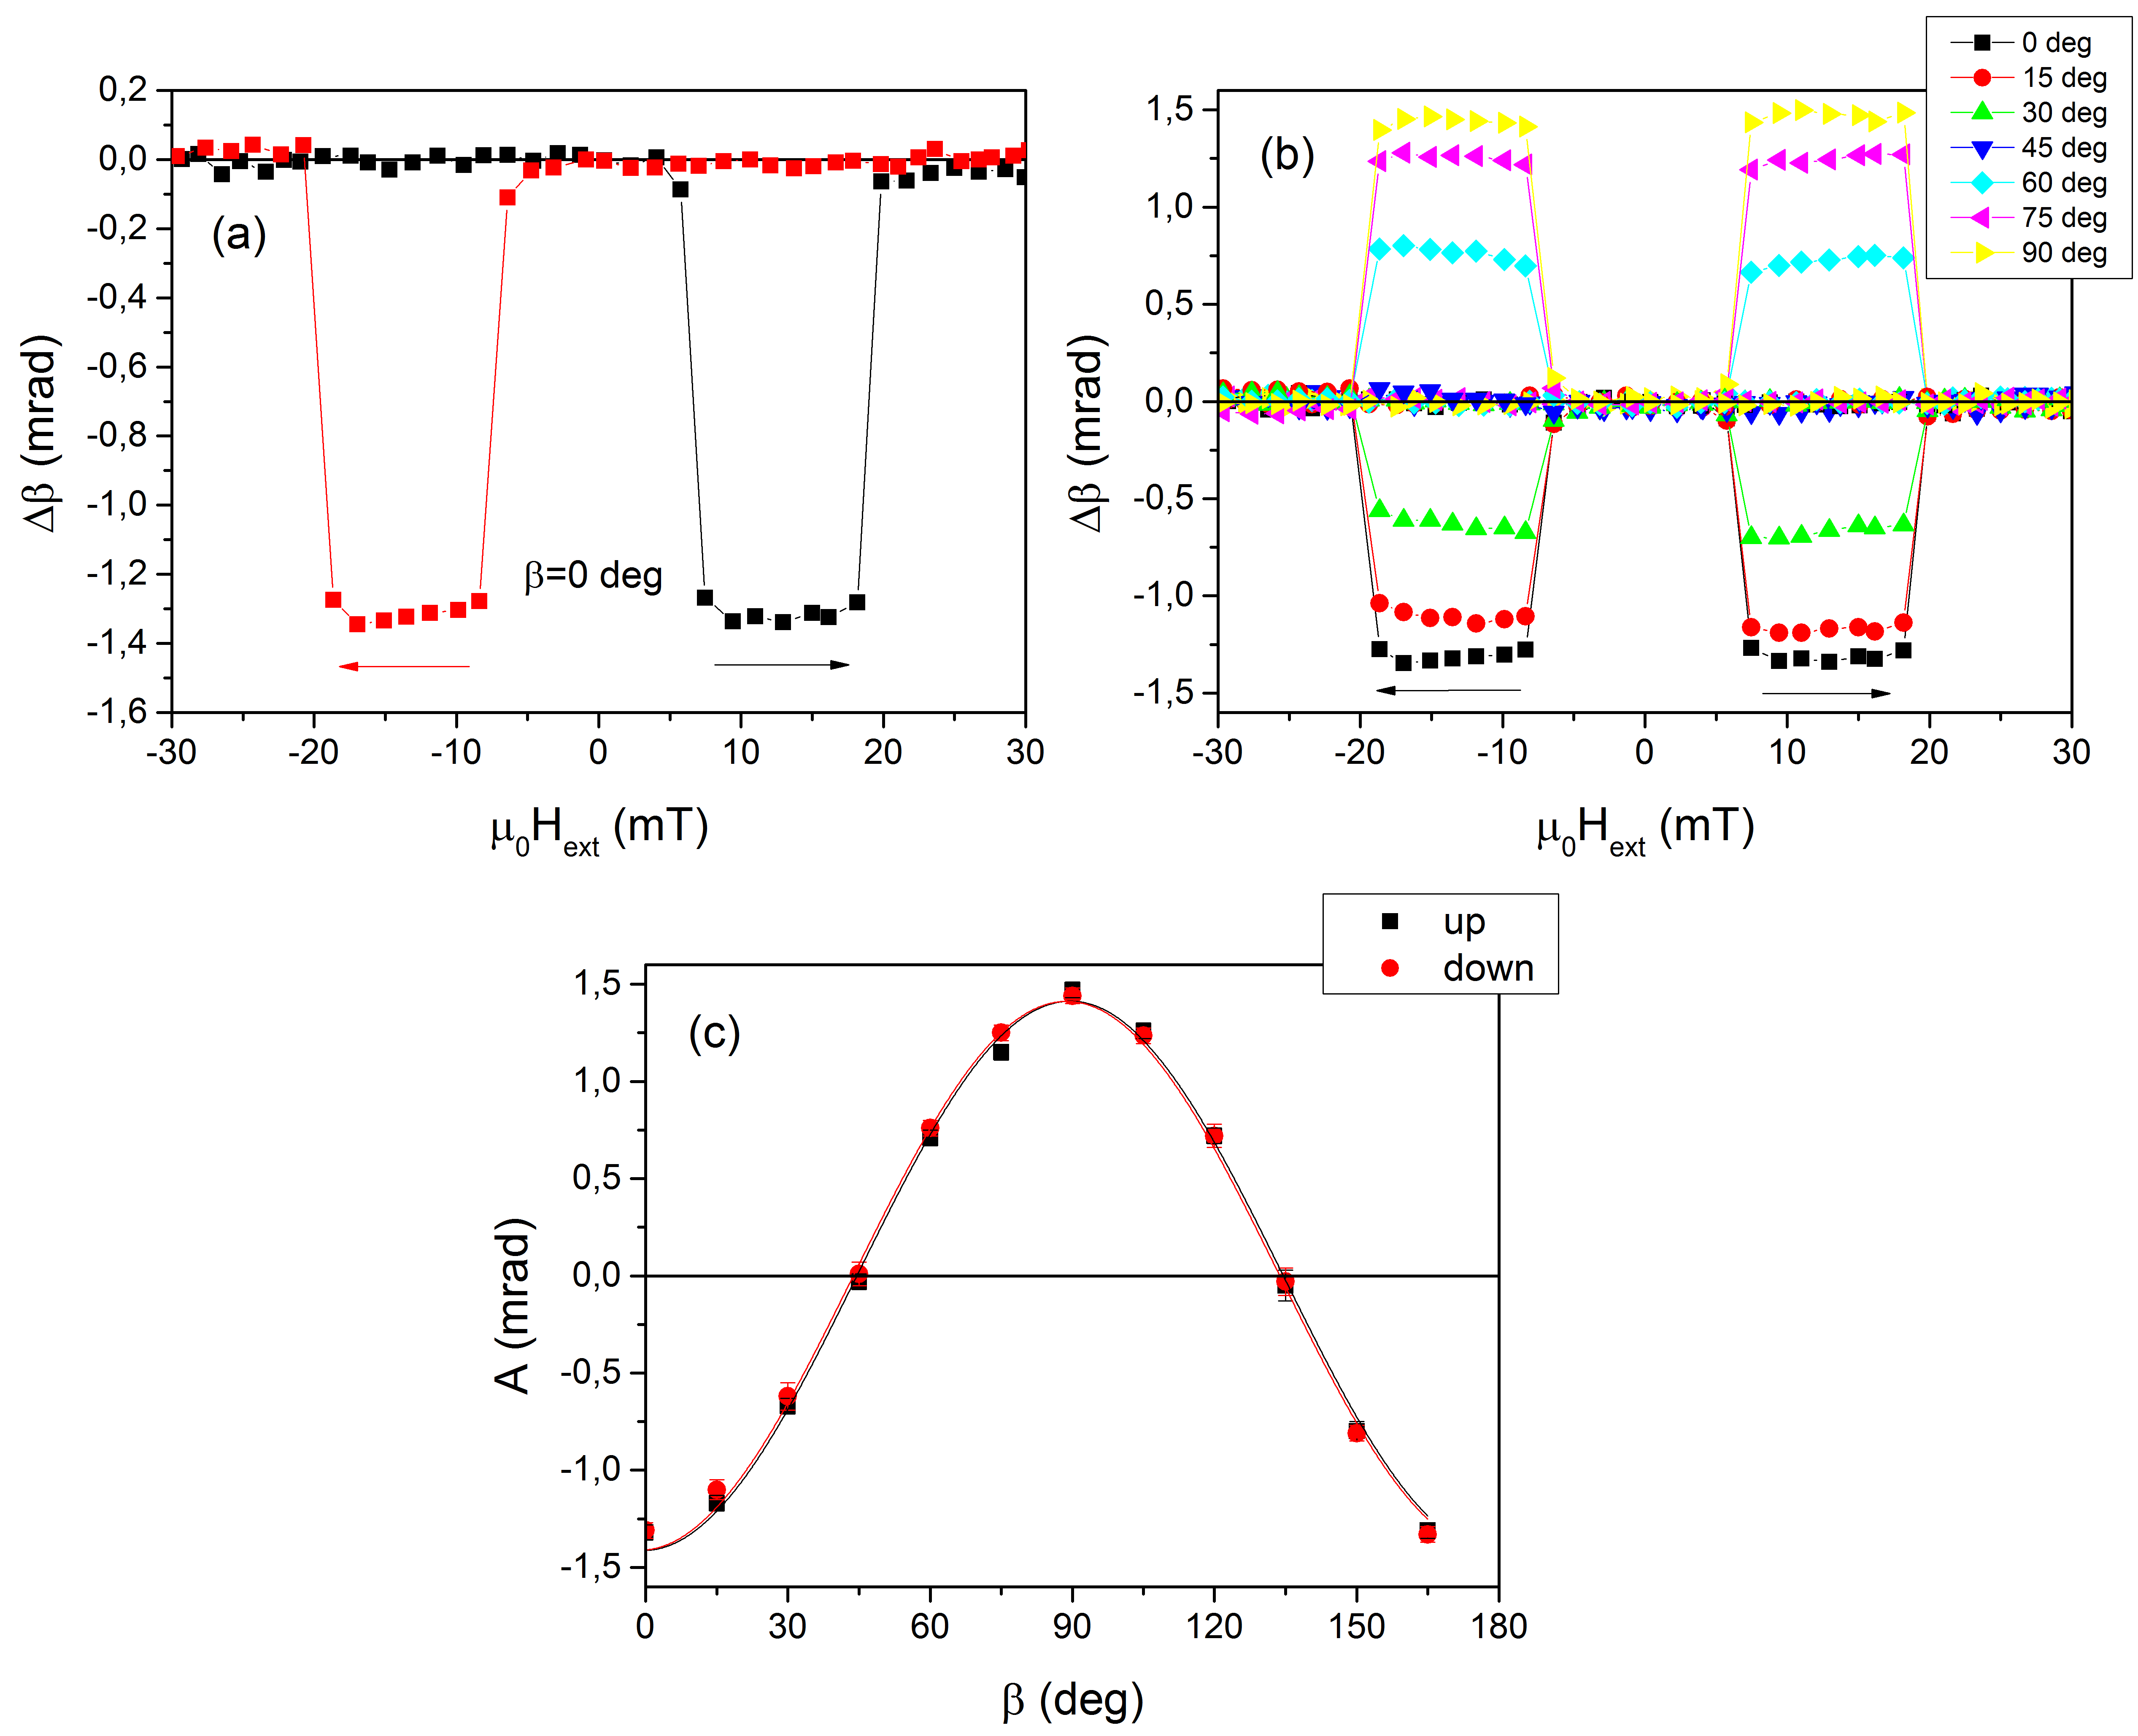
\includegraphics[width=\textwidth]{./png/nekolhyst_135pol_voigt}}
	\caption{Měření Voigtova jevu v hysterezních smyčkách pro $\phH=\ang{135}$ v~nekolineární geometrii. (a) Typická hysterezní smyčka ($\beta=\ang{0}$). (b) Polarizační závislost hysterezních smyček. (c) Polarizační závislost amplitudy $A$ (body), nafitovaná závislost vztahem \eqref{e:amplVoigt} (čára).}\label{nekol_vysledky_voigt}
\end{figure}

V součtovém napětí jsme také pozorovali obdobný signál. Měření probíhalo přibližně hodinu a během ní poměrně rovnoměrně a konzistentně klesala intenzita laseru. Nejdříve byla změřena polarizace $\beta=\ang{0}$ a poté jsme ji po \ang{15} zvyšovali až do $\beta=\ang{165}$. Na obr. \ref{nekol_vysledky_mld} (a) je graf, jak v průběhu měření klesala intenzita. To se projevilo i v samotných hysterezních smyčkách, viz obr. \ref{nekol_vysledky_mld} (b). Intenzita klesá s~časem, který má v up a down měřeních opačný směr.

Intenzita si během celého měření držela stejný trend poklesu, což nám umožnilo jednoduše porovnat hysterezní smyčky pro různé polarizace, viz obr. \ref{nekol_vysledky_mld} (c). Naměřené smyčky jsou vždy vydělené počáteční hodnotou a je odečtena 1 (takže při vyváženém můstku je $B=0$). Odečetli jsme amplitudy přeskoků $\Delta B$, její polarizační závislost je na obr. \ref{nekol_vysledky_mld} (d).

\begin{figure}[htbp]\centering
\qq{	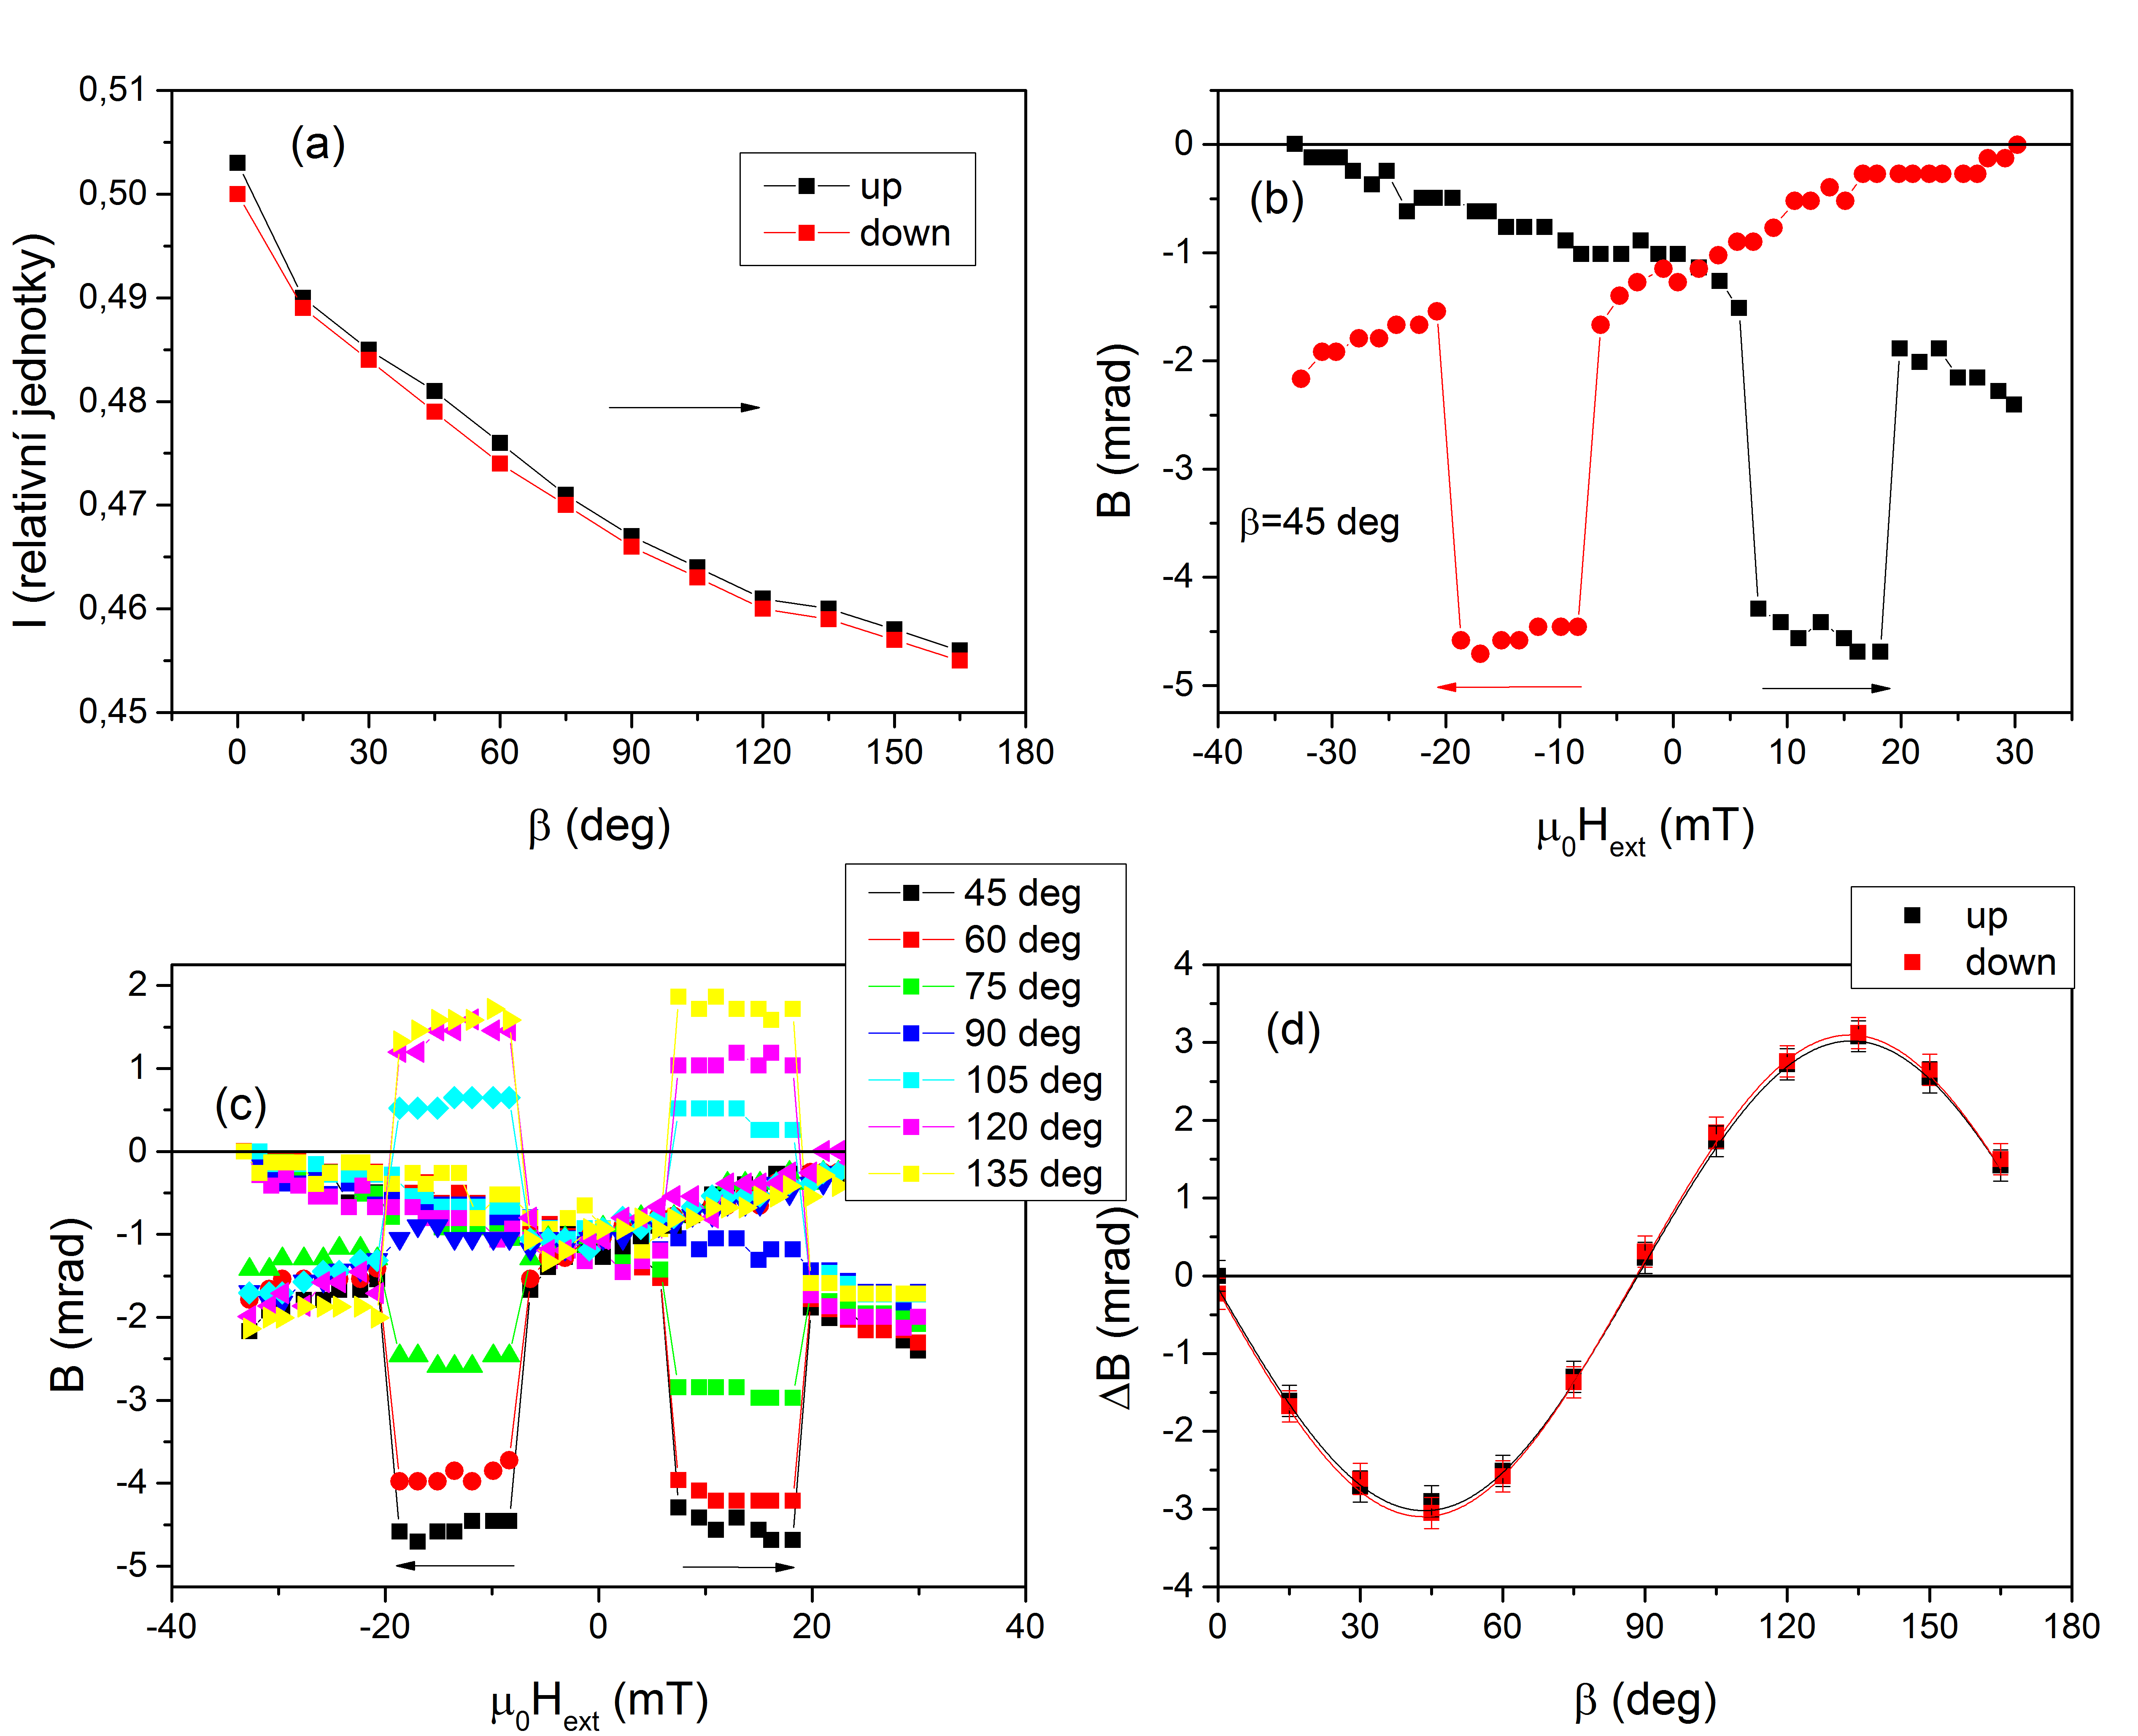
\includegraphics[width=\textwidth]{./png/nekolhyst_135pol_mld}}
	\caption{Měření MLD v hysterezních smyčkách pro $\phH=\ang{135}$ v nekolineární geometrii. (a) Průměrná intenzita laseru při měření jednotlivých polarizací. (b) Typická hysterezní smyčka ($\beta=\ang{45}$). (c) Polarizační závislost hysterezních smyček. (d) Polarizační závislost amplitudy $\Delta B$ (body), nafitovaná závislost vztahem \eqref{e:amplMLD} (čára).}\label{nekol_vysledky_mld}
\end{figure}


\FloatBarrier

\subsection*{Vnější pole ve směru \ang{0}}

V tomto směru se oproti $\phH=\ang{135}$ uplatňuje nový jev. Z obr. \ref{souradna_soustava_vzorek} (b) je vidět, že směr \ang{0} se ani přibližně neshoduje s žádnou snadnou osou magnetizace. Aplikací vnějšího pole $\hext$ dochází k vychýlení preferovaného směru magnetizace ze snadné osy. Vychýlení magnetizace závisí spojitě na intenzitě pole, což má za následek dodatečný magnetooptický signál. Hysterezní smyčku pak pozorujeme na trojúhelníkovém pozadí jako na obr. \ref{nekol_vysledky0_voigt} (a). Tento jev charakterizujeme hodnotou $A_r$, kterou definujeme jako (viz obr. \ref{zpracovani})
\begin{equation} \label{e:Ar}
A_{r}:=\Delta \beta_\text{vyvážený můstek} - \Delta \beta_{\hext=0} \,.
\end{equation}
Polarizační závislost $A_r$ je na obr. \ref{nekol_vysledky0_voigt} (c).
$A_r (\beta)$ jsme také proložili funkcí $a\sin(\beta-b)$ s parametry $a$, $b$.

Amplitudu přeskoku $A$ určíme z grafu vzhledem k interpolovanému pozadí zmiňovaného jevu.


\begin{figure}[htbp]\centering
\qq{	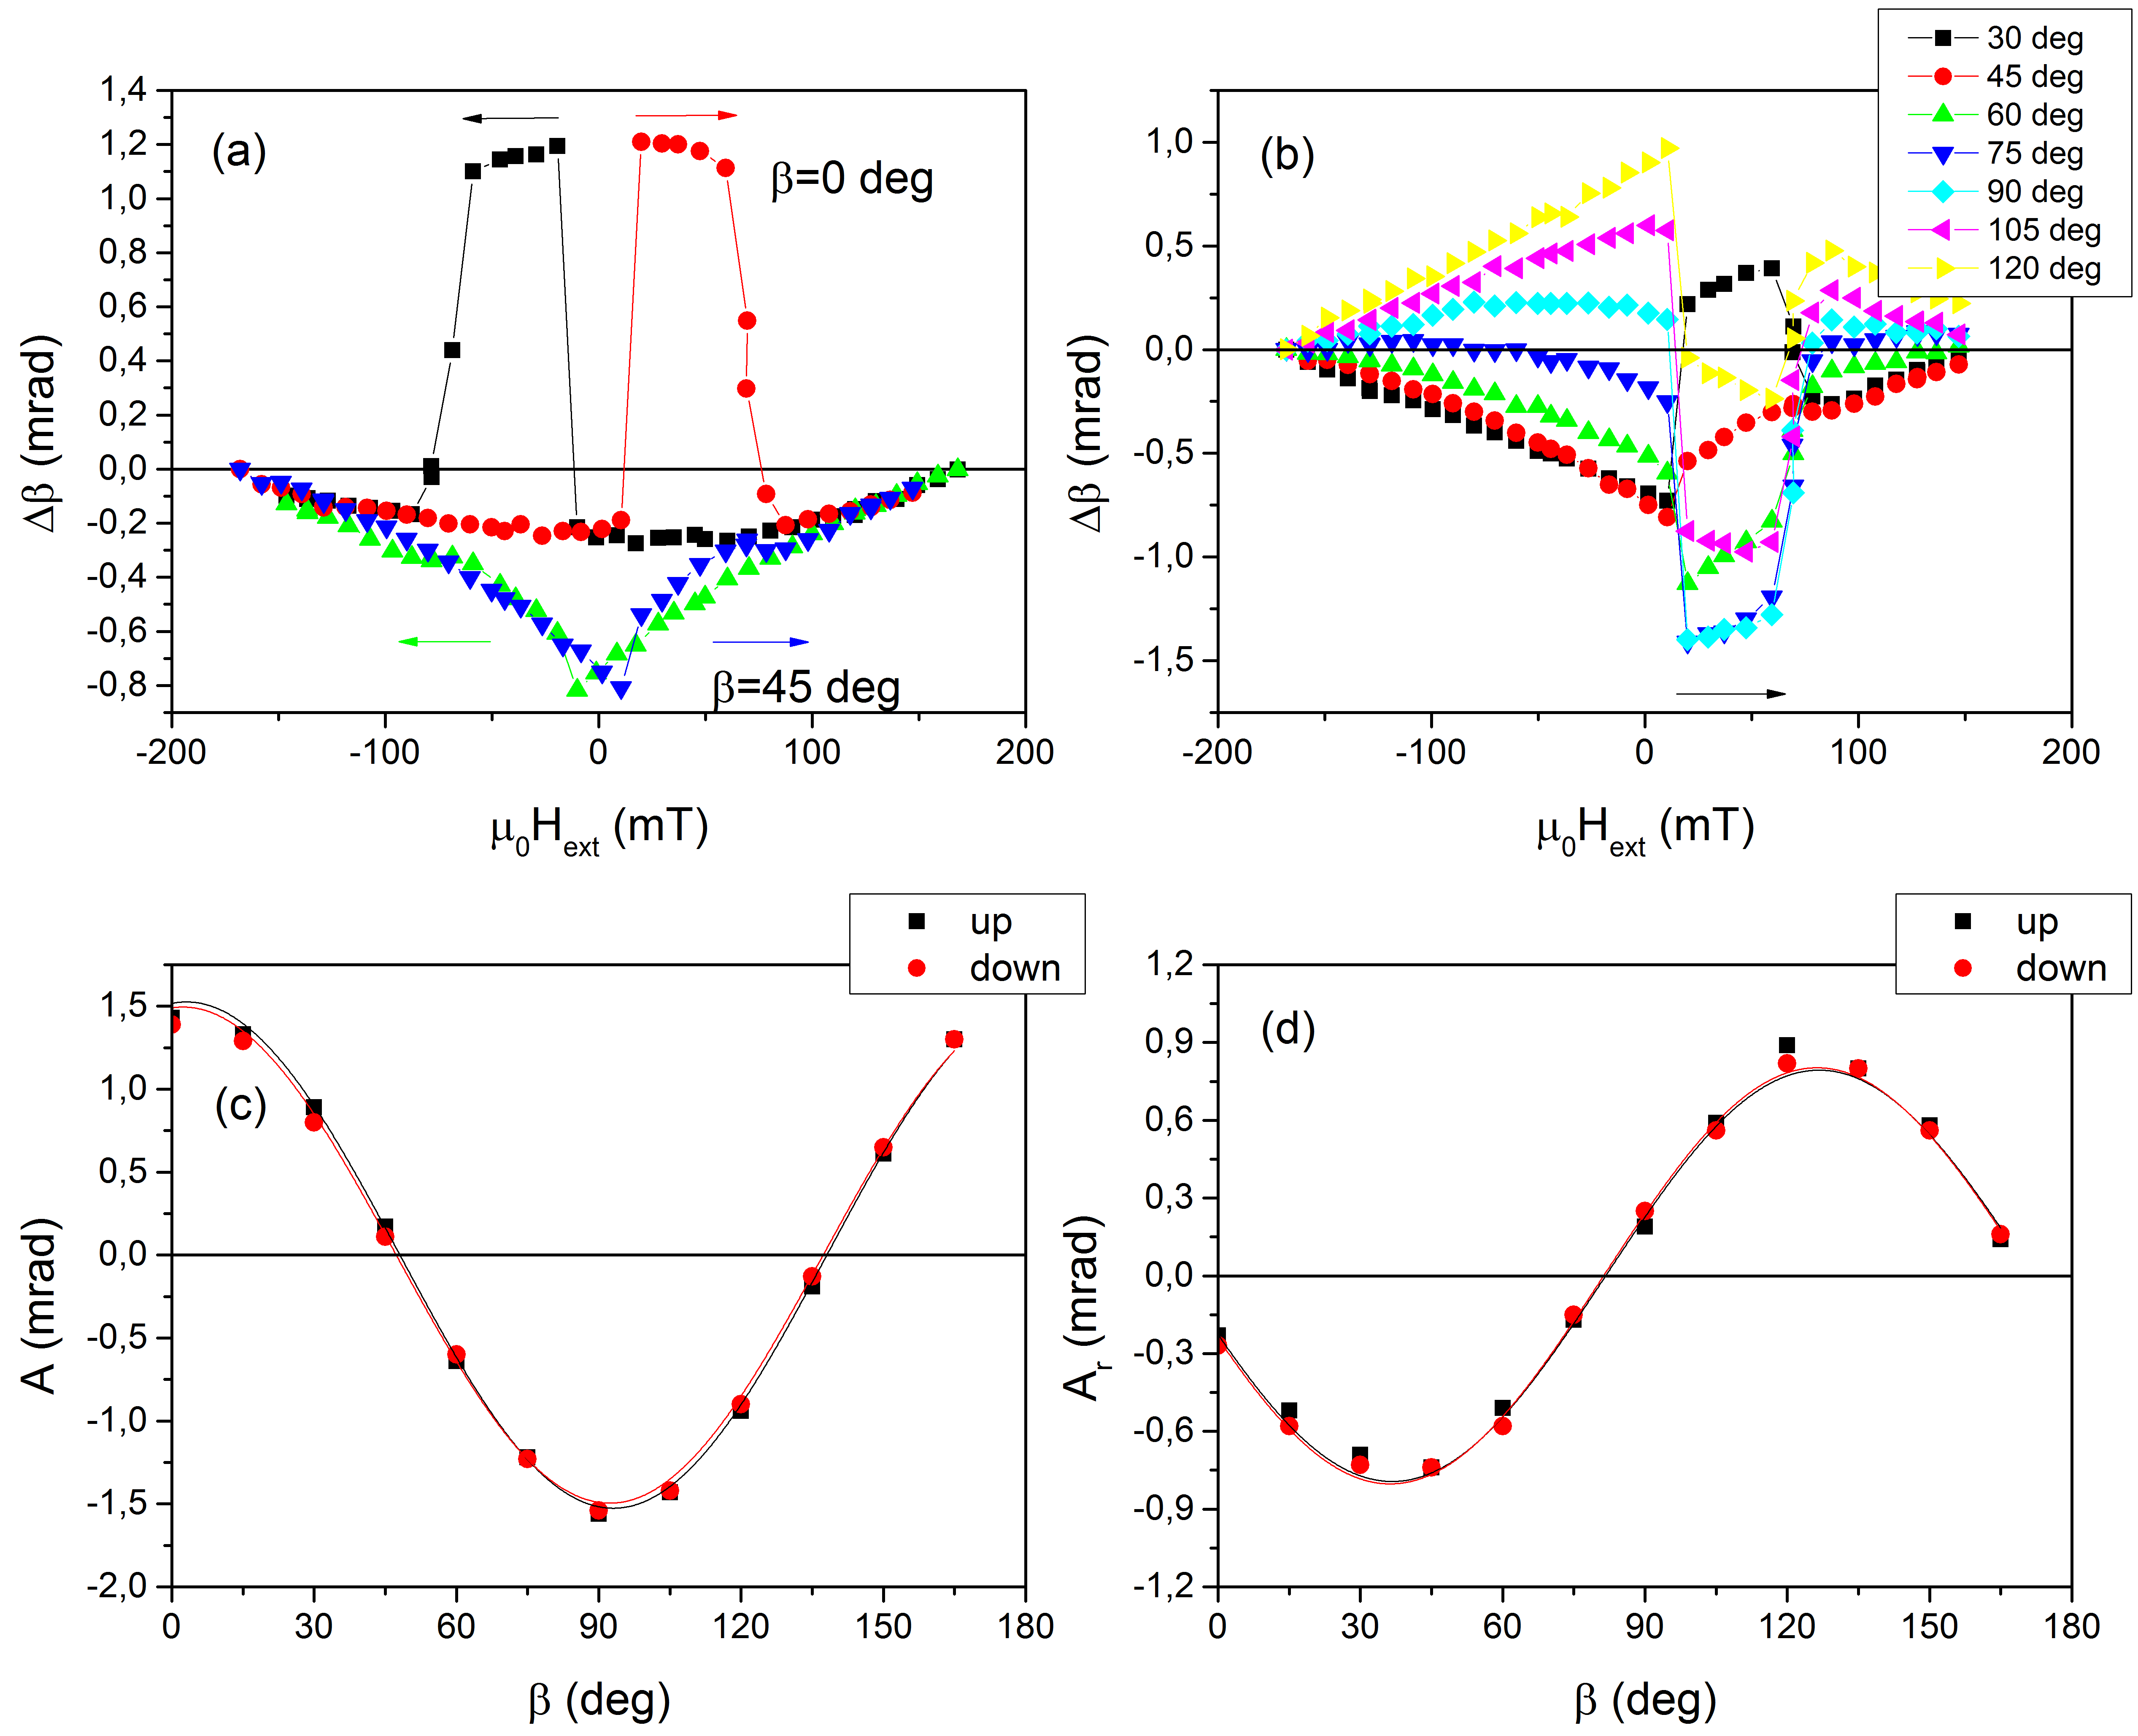
\includegraphics[width=\textwidth]{./png/nekolhyst_0pol_voigt}}
	\caption{Měření Voigtova jevu v hysterezních smyčkách pro $\phH=\ang{0}$ v nekolineární geometrii. (a) Typická hysterezní smyčka ($\beta=\ang{0}$ a \ang{45}). (b) Hysterezní smyčky pro vybrané polarizace. (c) Polarizační závislost amplitudy přeskoku $A$ (body), nafitovaná závislost vztahem \eqref{e:amplVoigt} (čára). (d) Polarizační závislost $A_r$ (body), nafitovaná závislost funkcí $a\sin(\beta-b)$ (čára).}\label{nekol_vysledky0_voigt}
\end{figure}

V součtovém signálu jsou opět zřetelné hysterezní smyčky na pozadí stále klesající intenzity. Data jsme zpracovali stejným způsobem jako pro $\phH=\ang{135}$. Naměřená data jsou na obr. \ref{nekol_vysledky0_mld} (a-d). Jev s trojúhelníkovým profilem je opět přítomný (viz obr. \ref{nekol_vysledky0_mld} (c)), ale na pozadí klesající intenzity je obtížné ho dobře změřit.

Na tomto místě je vhodné poznamenat, že data naměřená pro $\phH=\ang{135}$ a \ang{0} mají stejnou symetrii (tj. polohu extrémů a uzlových bodů), ale liší se jejich znaménko (viz např. obr. \ref{nekol_vysledky_voigt} (c) a \ref{nekol_vysledky0_voigt} (c)).

\begin{figure}[htbp]\centering
\qq{	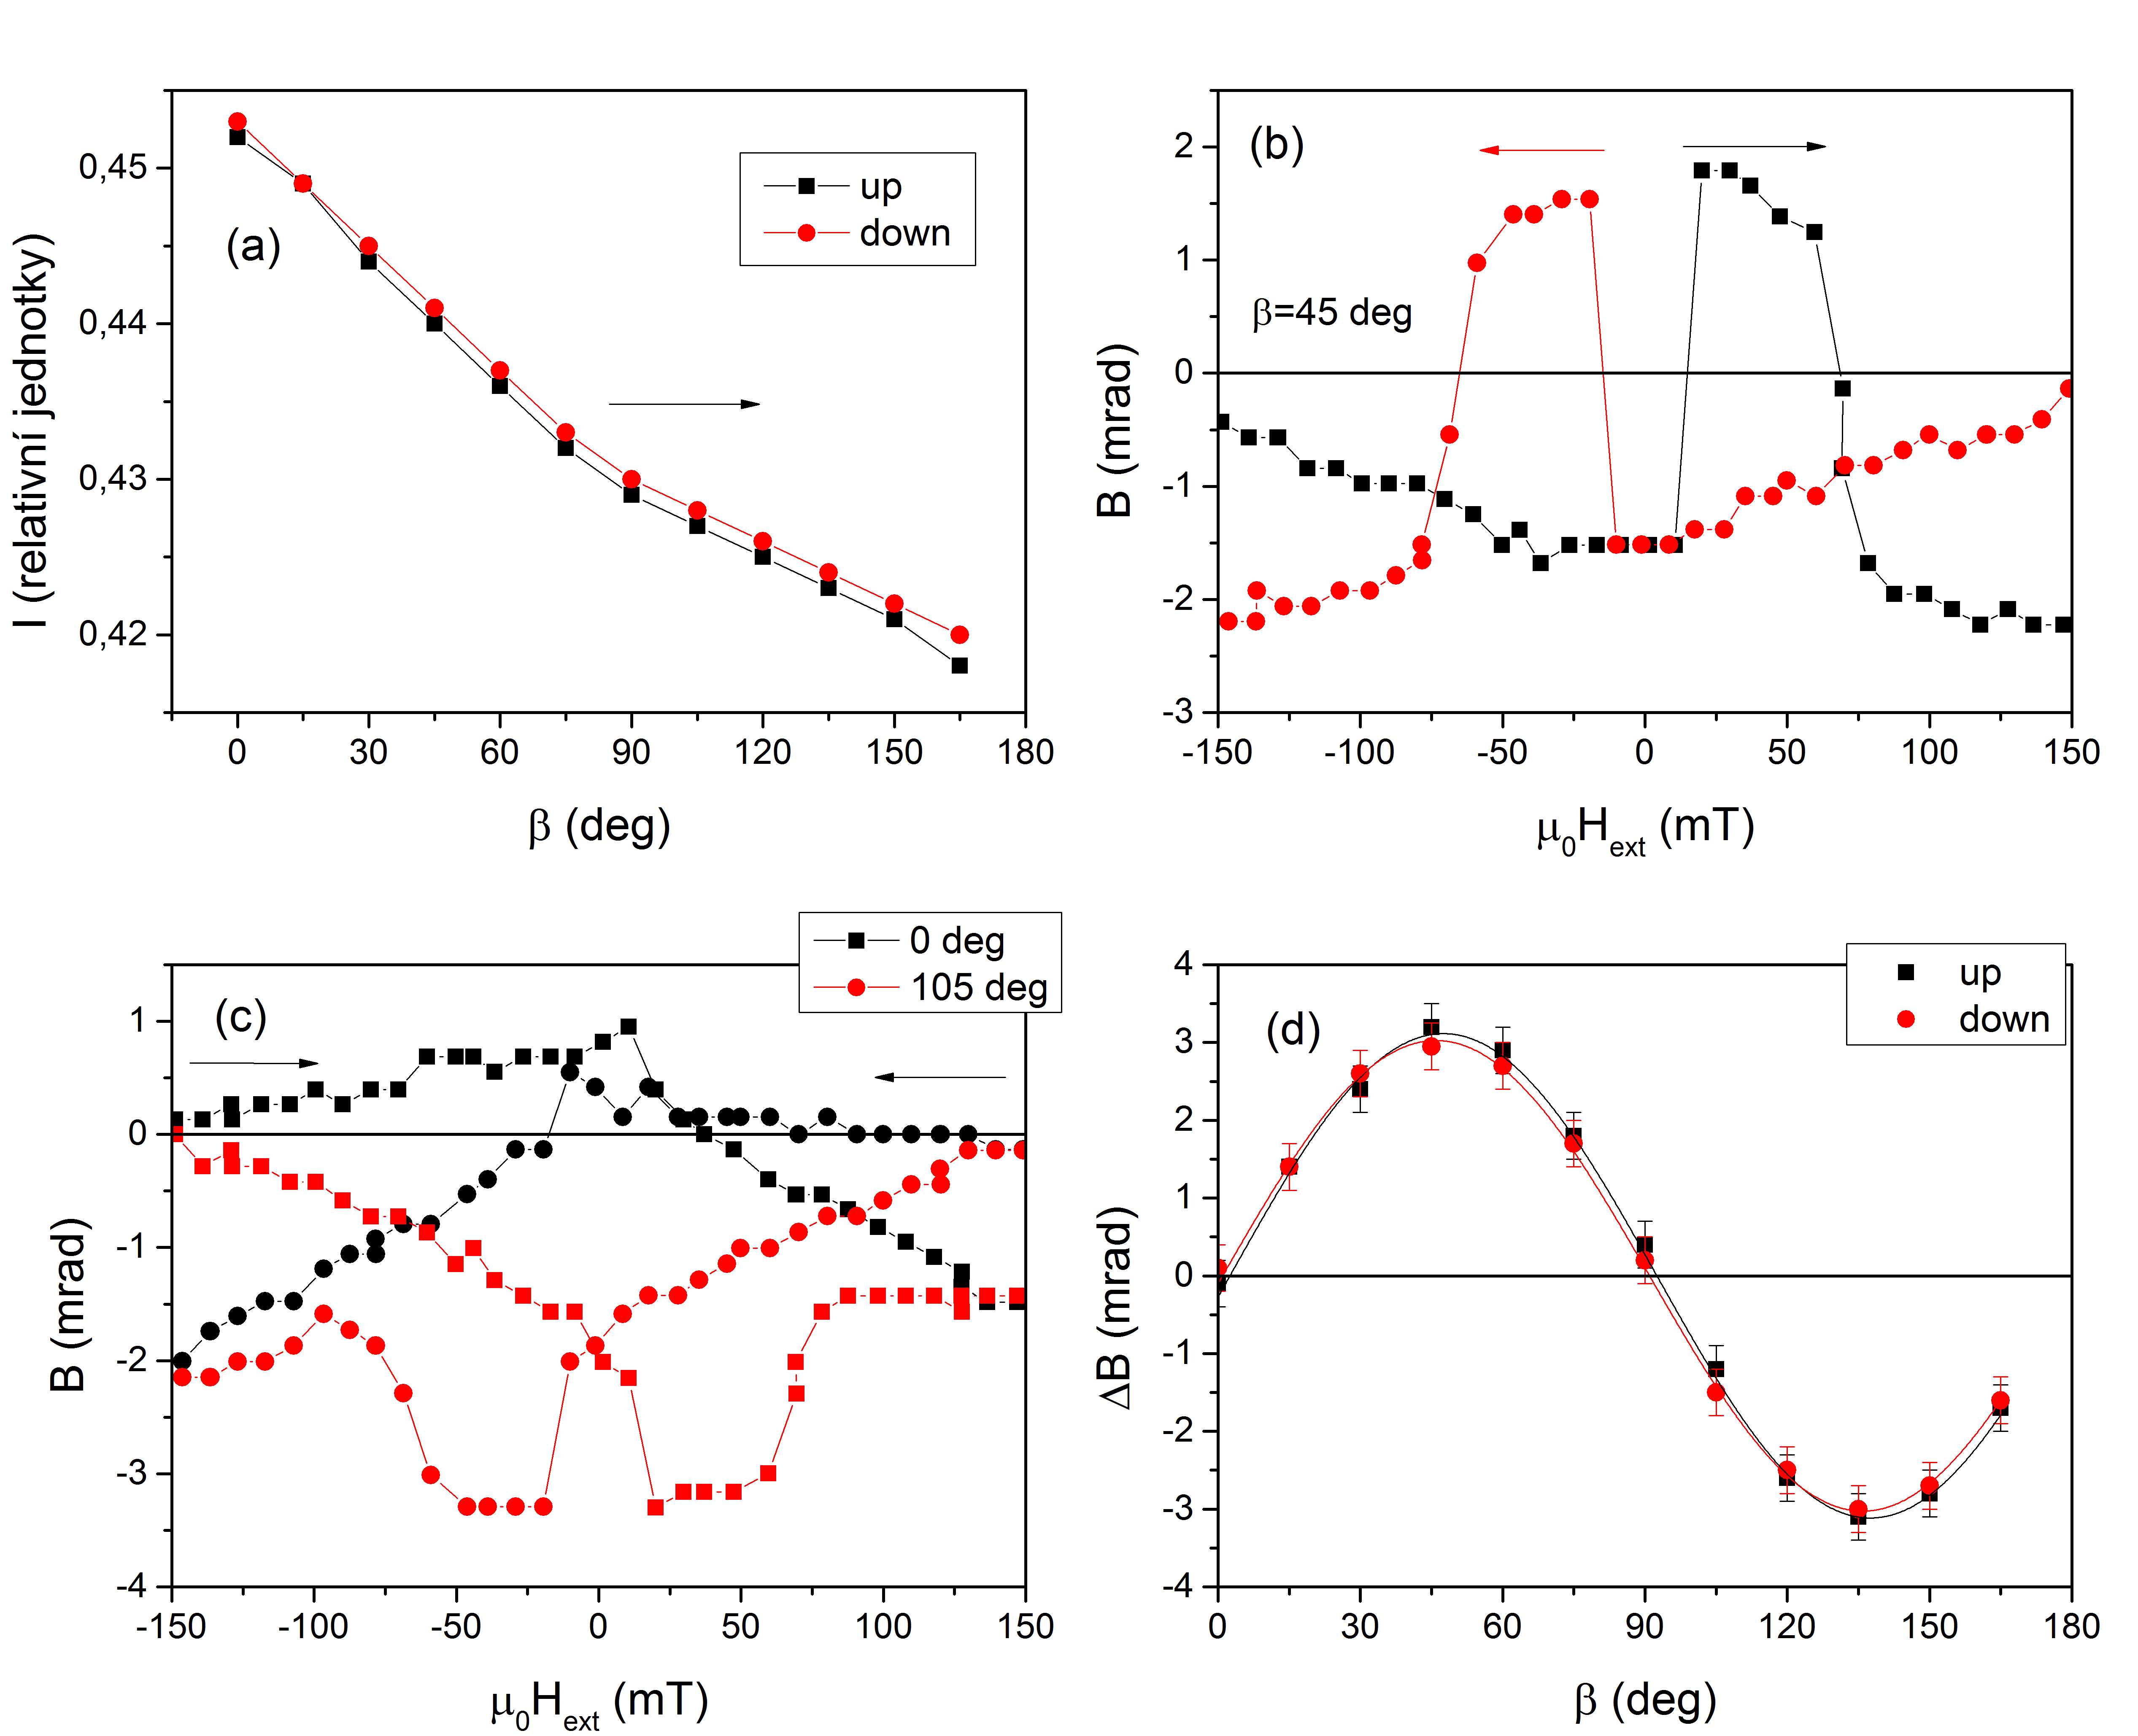
\includegraphics[width=\textwidth]{./png/nekolhyst_0pol_mld}}
	\caption{Měření MLD v hysterezních smyčkách pro $\phH=\ang{0}$ v nekolineární geometrii. (a) Průměrná intenzita laseru při měření jednotlivých polarizací. (b) Typická hysterezní smyčka ($\beta=\ang{0}$). (c) Vybrané hysterezní smyčky $\beta=\ang{0}$, \ang{105}. (d) Polarizační závislost amplitudy $\Delta B$ (body), nafitovaná závislost vztahem \eqref{e:amplMLD} (čára).}\label{nekol_vysledky0_mld}
\end{figure}

V tabulce \ref{tab_nekol_hyst} uvádíme souhrn fitováním určených hodnot jednotlivých parametrů ve vztazích \eqref{e:amplVoigt} a \eqref{e:amplMLD}.


\begin{table}[htbp]	
	\centering	
	\begin{tabular}{c||cc|cc|cc}
		& & & \multicolumn{2}{c|}{fit Voigtův jev} & \multicolumn{2}{c}{fit MLD} \\
		$\phH$ & $\mu_0\hcj$ & $\mu_0\hcd$ & $\pmld \sin\xi$ & $\gamma$ & $\pmld \sin\xi$ & $\gamma$ \\
		(deg) & (mT) & (mT) & (\si{\milli\radian}) & (deg) & (\si{\milli\radian}) & (deg) \\ \hline
		135 up & \num{5,5(4)} & \num{19,0(5)} & \num{-0,70(5)} & \num{89.5(10)} & \num{-0,75(4)} & \num{88,5(10)} \\
		135 down & \num{5,8(4)} & \num{19,8(8)} & \num{-0,70(5)} & \num{88,8(15)} & \num{-0,77(4)} & \num{88,2(10)} \\ \hline
		0 up & \num{15,0(40)} & \num{83(4)} & \num{-0,76(4)} & \num{93,1(10)}& \num{-0,78(5)} & \num{92,5(15)} \\
		0 down & \num{14,5(40)} & \num{81(3)} & \num{-0,75(5)} & \num{92,3(15)} & \num{-0,76(4)}& \num{90,9(10)} \\
	\end{tabular}
	\caption{Měření hysterezních smyček v nekolineární geometrii. U $\phH=\ang{135}$ jsme změnili znaménko $\pmld \sin\xi$, protože dochází k přeskoku v opačném směru než předpokládají vztahy \eqref{e:amplVoigt} a \eqref{e:amplMLD}. V tomto případě platí stejný vztah s~opačným znaménkem.}
	\label{tab_nekol_hyst}
\end{table}

Z této tabulky je patrné, že veškeré získané hodnoty jsou v rámci chyby stejné. Dále je z tohoto měření možné určit, s jakou přesností byl vzorek skutečně nalepen v požadované orientaci --- situaci znázorněné na obr. \ref{souradna_soustava_vzorek} totiž odpovídá $\gamma=\ang{90}$ a průměrná experimentálně určená hodnota $\gamma=\num{90,5(17)}^\circ$.


\FloatBarrier
\section{Kolineární geometrie} \label{kap_kolinearni}
V kolineární geometrii jsme provedli tři druhy měření hysterezních smyček. 
\begin{itemize}
\item Polarizační závislost pro $\phH=\ang{135}$ a $T<\SI{15}{\kelvin}$ pro ověření funkčnosti a porovnání s nekolineární geometrií.
\item Závislost na směru vnějšího pole $\phH \in (\ang{0},\ang{360})$ při $T<\SI{15}{\kelvin}$ a fixovaném $\gamma-\beta=\ang{90}$ (maximální Voigtův jev a nulové MLD).
\item Teplotní závislost pro $\phH=\ang{135}$ a fixované polarizaci $\beta=\ang{0}$ (maximální Voigtův jev a nulové MLD).
\end{itemize}


\subsection{Polarizační závislost při vnějším poli ve směru \ang{135}}
Měření proběhlo při teplotě $T<\SI{15}{\kelvin}$ a intenzita laseru dopadajícího na vzorek byla \SI{2}{\milli\watt}.

Na obr. \ref{kol_vysledky_voigt} (a) je typický průběh Voigtova jevu. Na obr. \ref{kol_vysledky_voigt} (b) jsou hysterezní smyčky pro několik vybraných polarizací. Polarizační závislost amplitudy přeskoku $A$ je vykreslena na obr. \ref{kol_vysledky_voigt} (c). V tabulce \ref{tab_kol_hyst135} jsou shrnuté získané výsledky.

\begin{figure}[htbp]\centering
\qq{	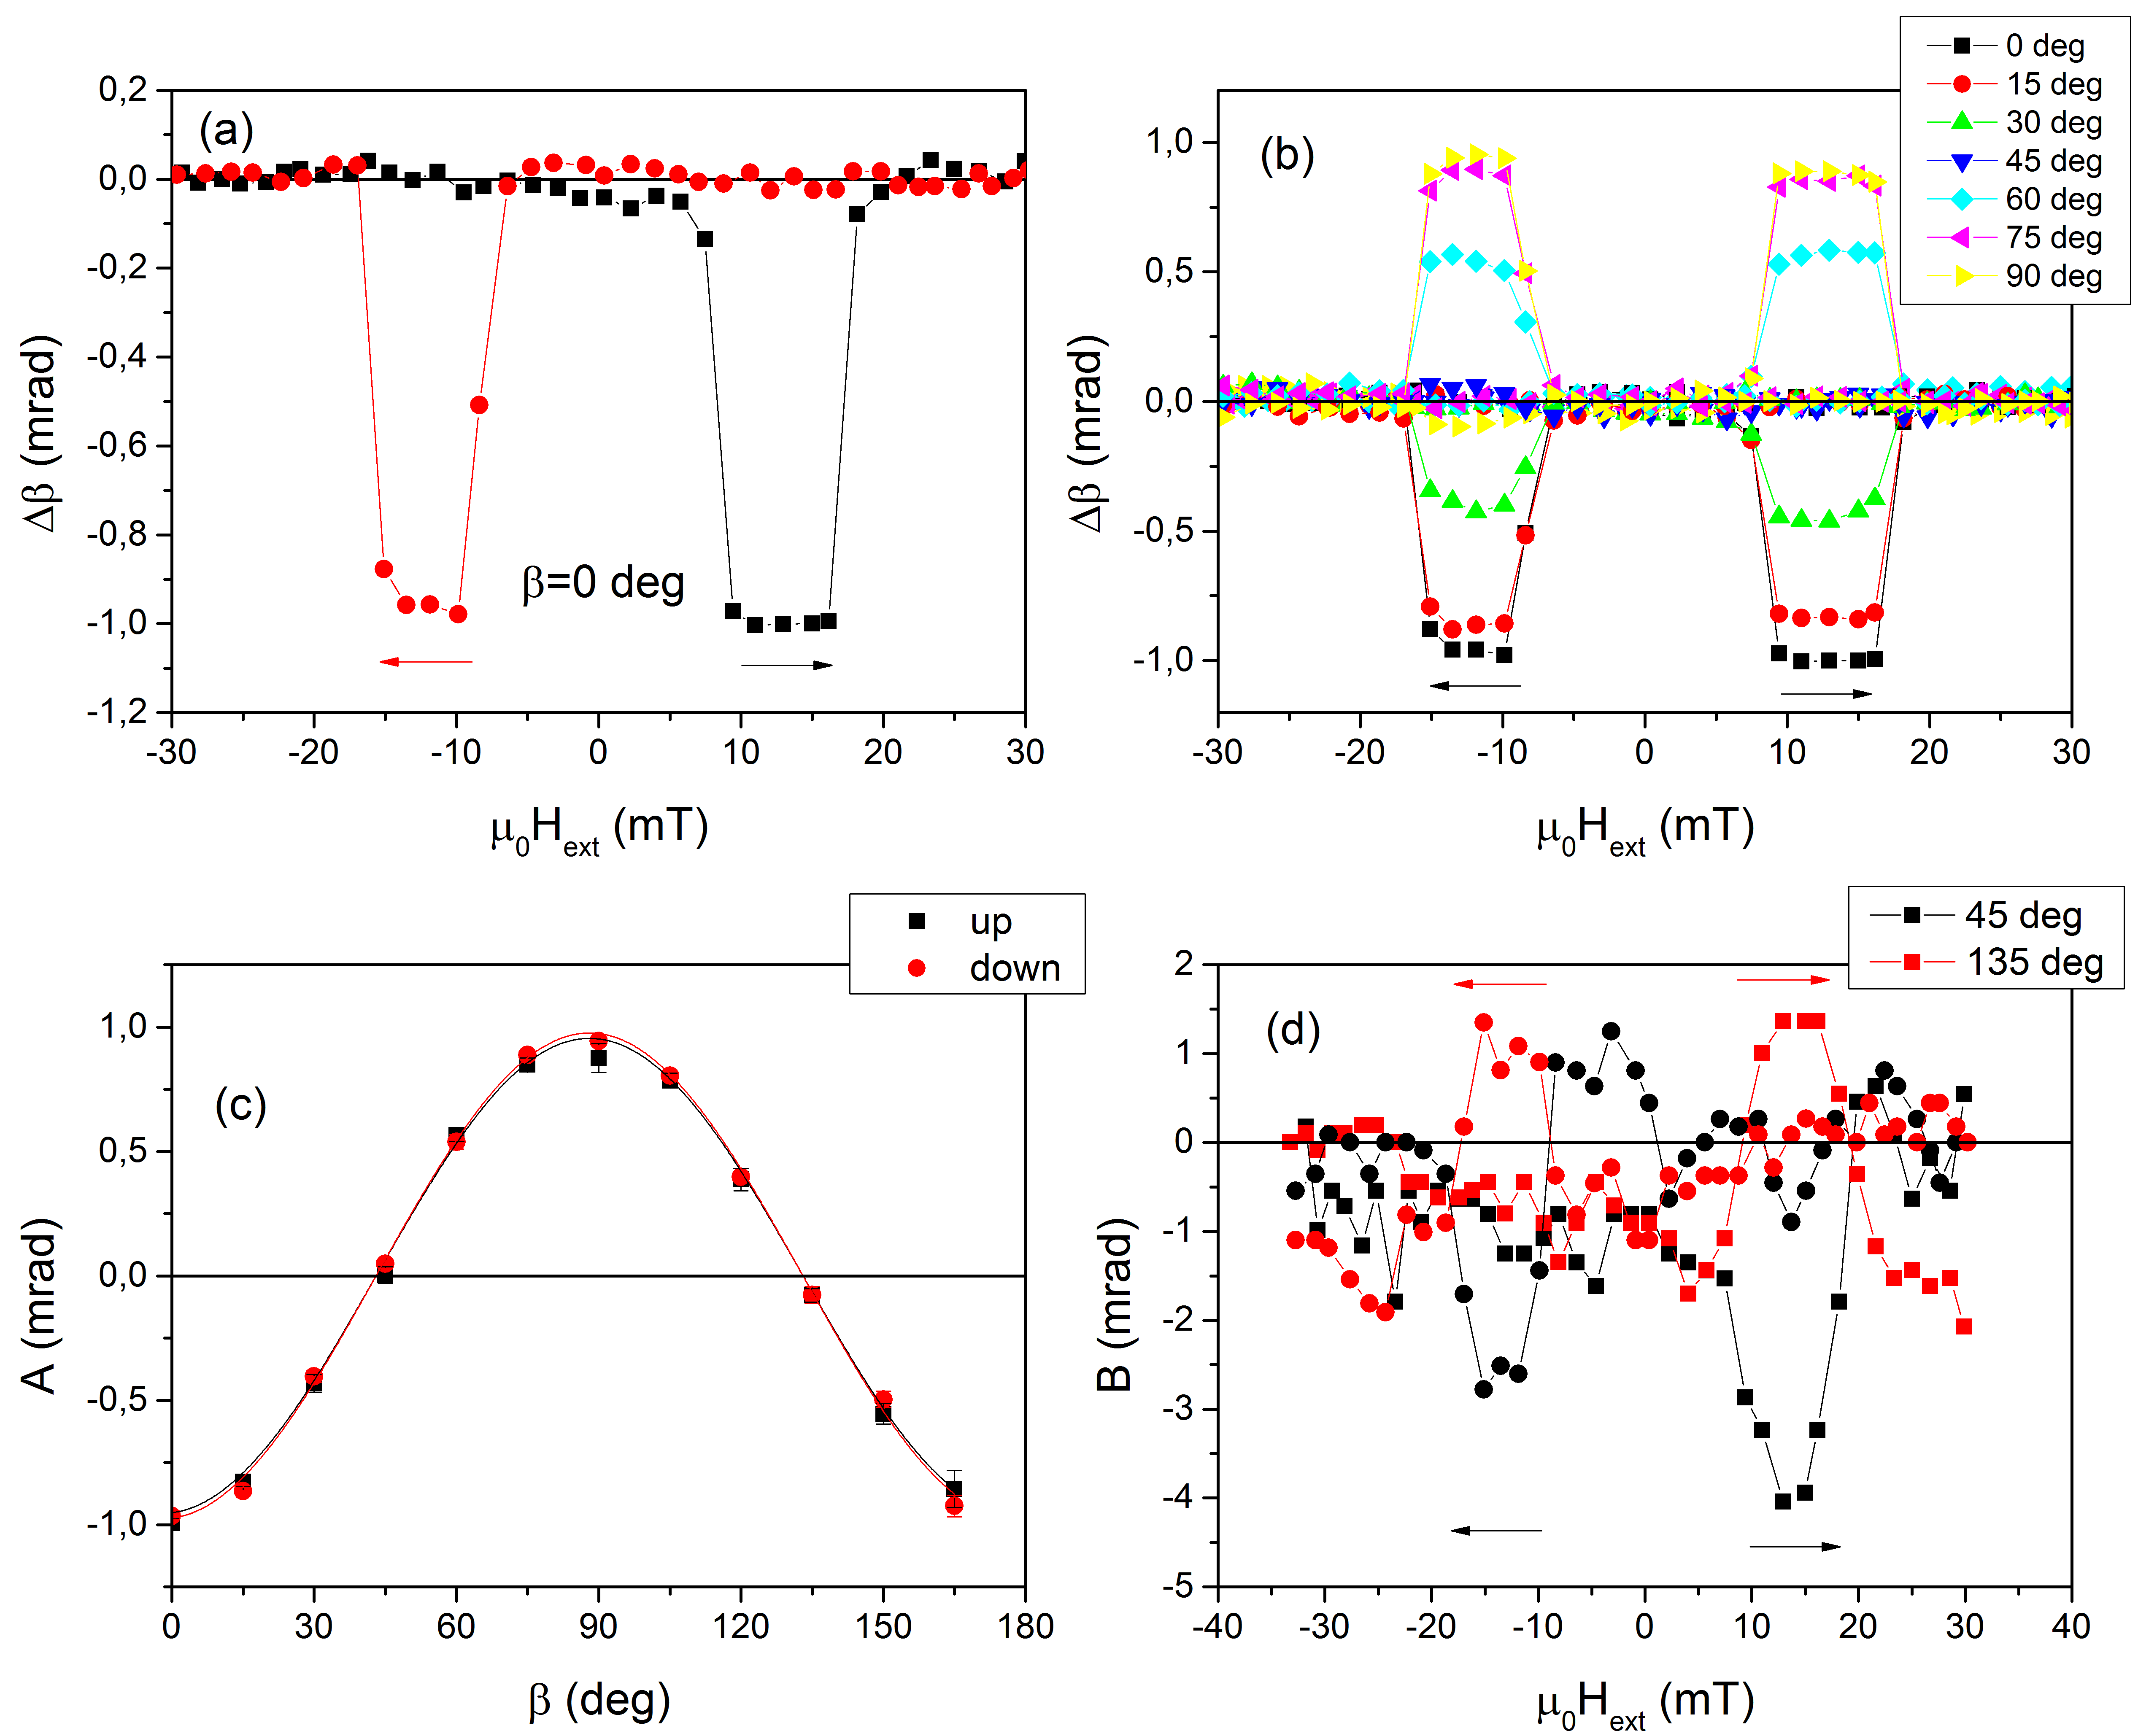
\includegraphics[width=\textwidth]{./png/kolhyst_135pol}}
	\caption{Měření Voigtova jevu v hysterezních smyčkách pro $\phH=\ang{135}$ v~kolineární geometrii. (a) Typická hysterezní smyčka ($\beta=\ang{0}$). (b) Polarizační závislost hysterezních smyček. (c) Polarizační závislost amplitudy $A$ (body), nafitovaná závislost vztahem \eqref{e:amplVoigt} (čára). (d) Součtový signál pro vybrané polarizace.}\label{kol_vysledky_voigt}
\end{figure}

\begin{table}[htbp]	
	\centering	
	\begin{tabular}{c||cc|cc}
		& & & \multicolumn{2}{c}{fit Voigtův jev} \\
		 & $\mu_0\hcj$ & $\mu_0\hcd$ & $\pmld \sin\xi$ & $\gamma$ \\
		 & (mT) & (mT) & (\si{\milli\radian}) & (deg)  \\ \hline
		up & \num{6,8(4)} & \num{17,6(6)} & \num{-0,48(4)} & \num{88,1(15)} \\
		down & \num{7,1(6)} & \num{16,5(7)} & \num{-0,49(3)} & \num{88,1(10)} \\
	\end{tabular}
	\caption{Měření hysterezních smyček v kolineární geometrii pro $\phH=\ang{135}$. Změnili jsme znaménko $\pmld \sin\xi$, protože dochází k přeskoku v opačném směru než předpokládá vztah \eqref{e:amplVoigt}}
	\label{tab_kol_hyst135}
\end{table}

V součtovém signálu je sice patrný MLD signál, ale je téměř na úrovni šumu a tak ho nezpracováváme, viz obr. \ref{kol_vysledky_voigt} (d). Vybrané polarizace jsou ty, u kterých by MLD mělo být nejsilnější.

Ve srovnání s měřením v nekolineární geometrii (viz obr. \ref{kol_nekol}) je patrné, že toto měření proběhlo při vyšší teplotě (viz níže). Koercitivní pole jsou nižší a $|\pmld|$ také. To mohlo být způsobeno, kromě odlišného zchlazení vzorku kryostatem, také vyšším výkonem použitého laseru.

\begin{figure}[htbp]\centering
\qq{	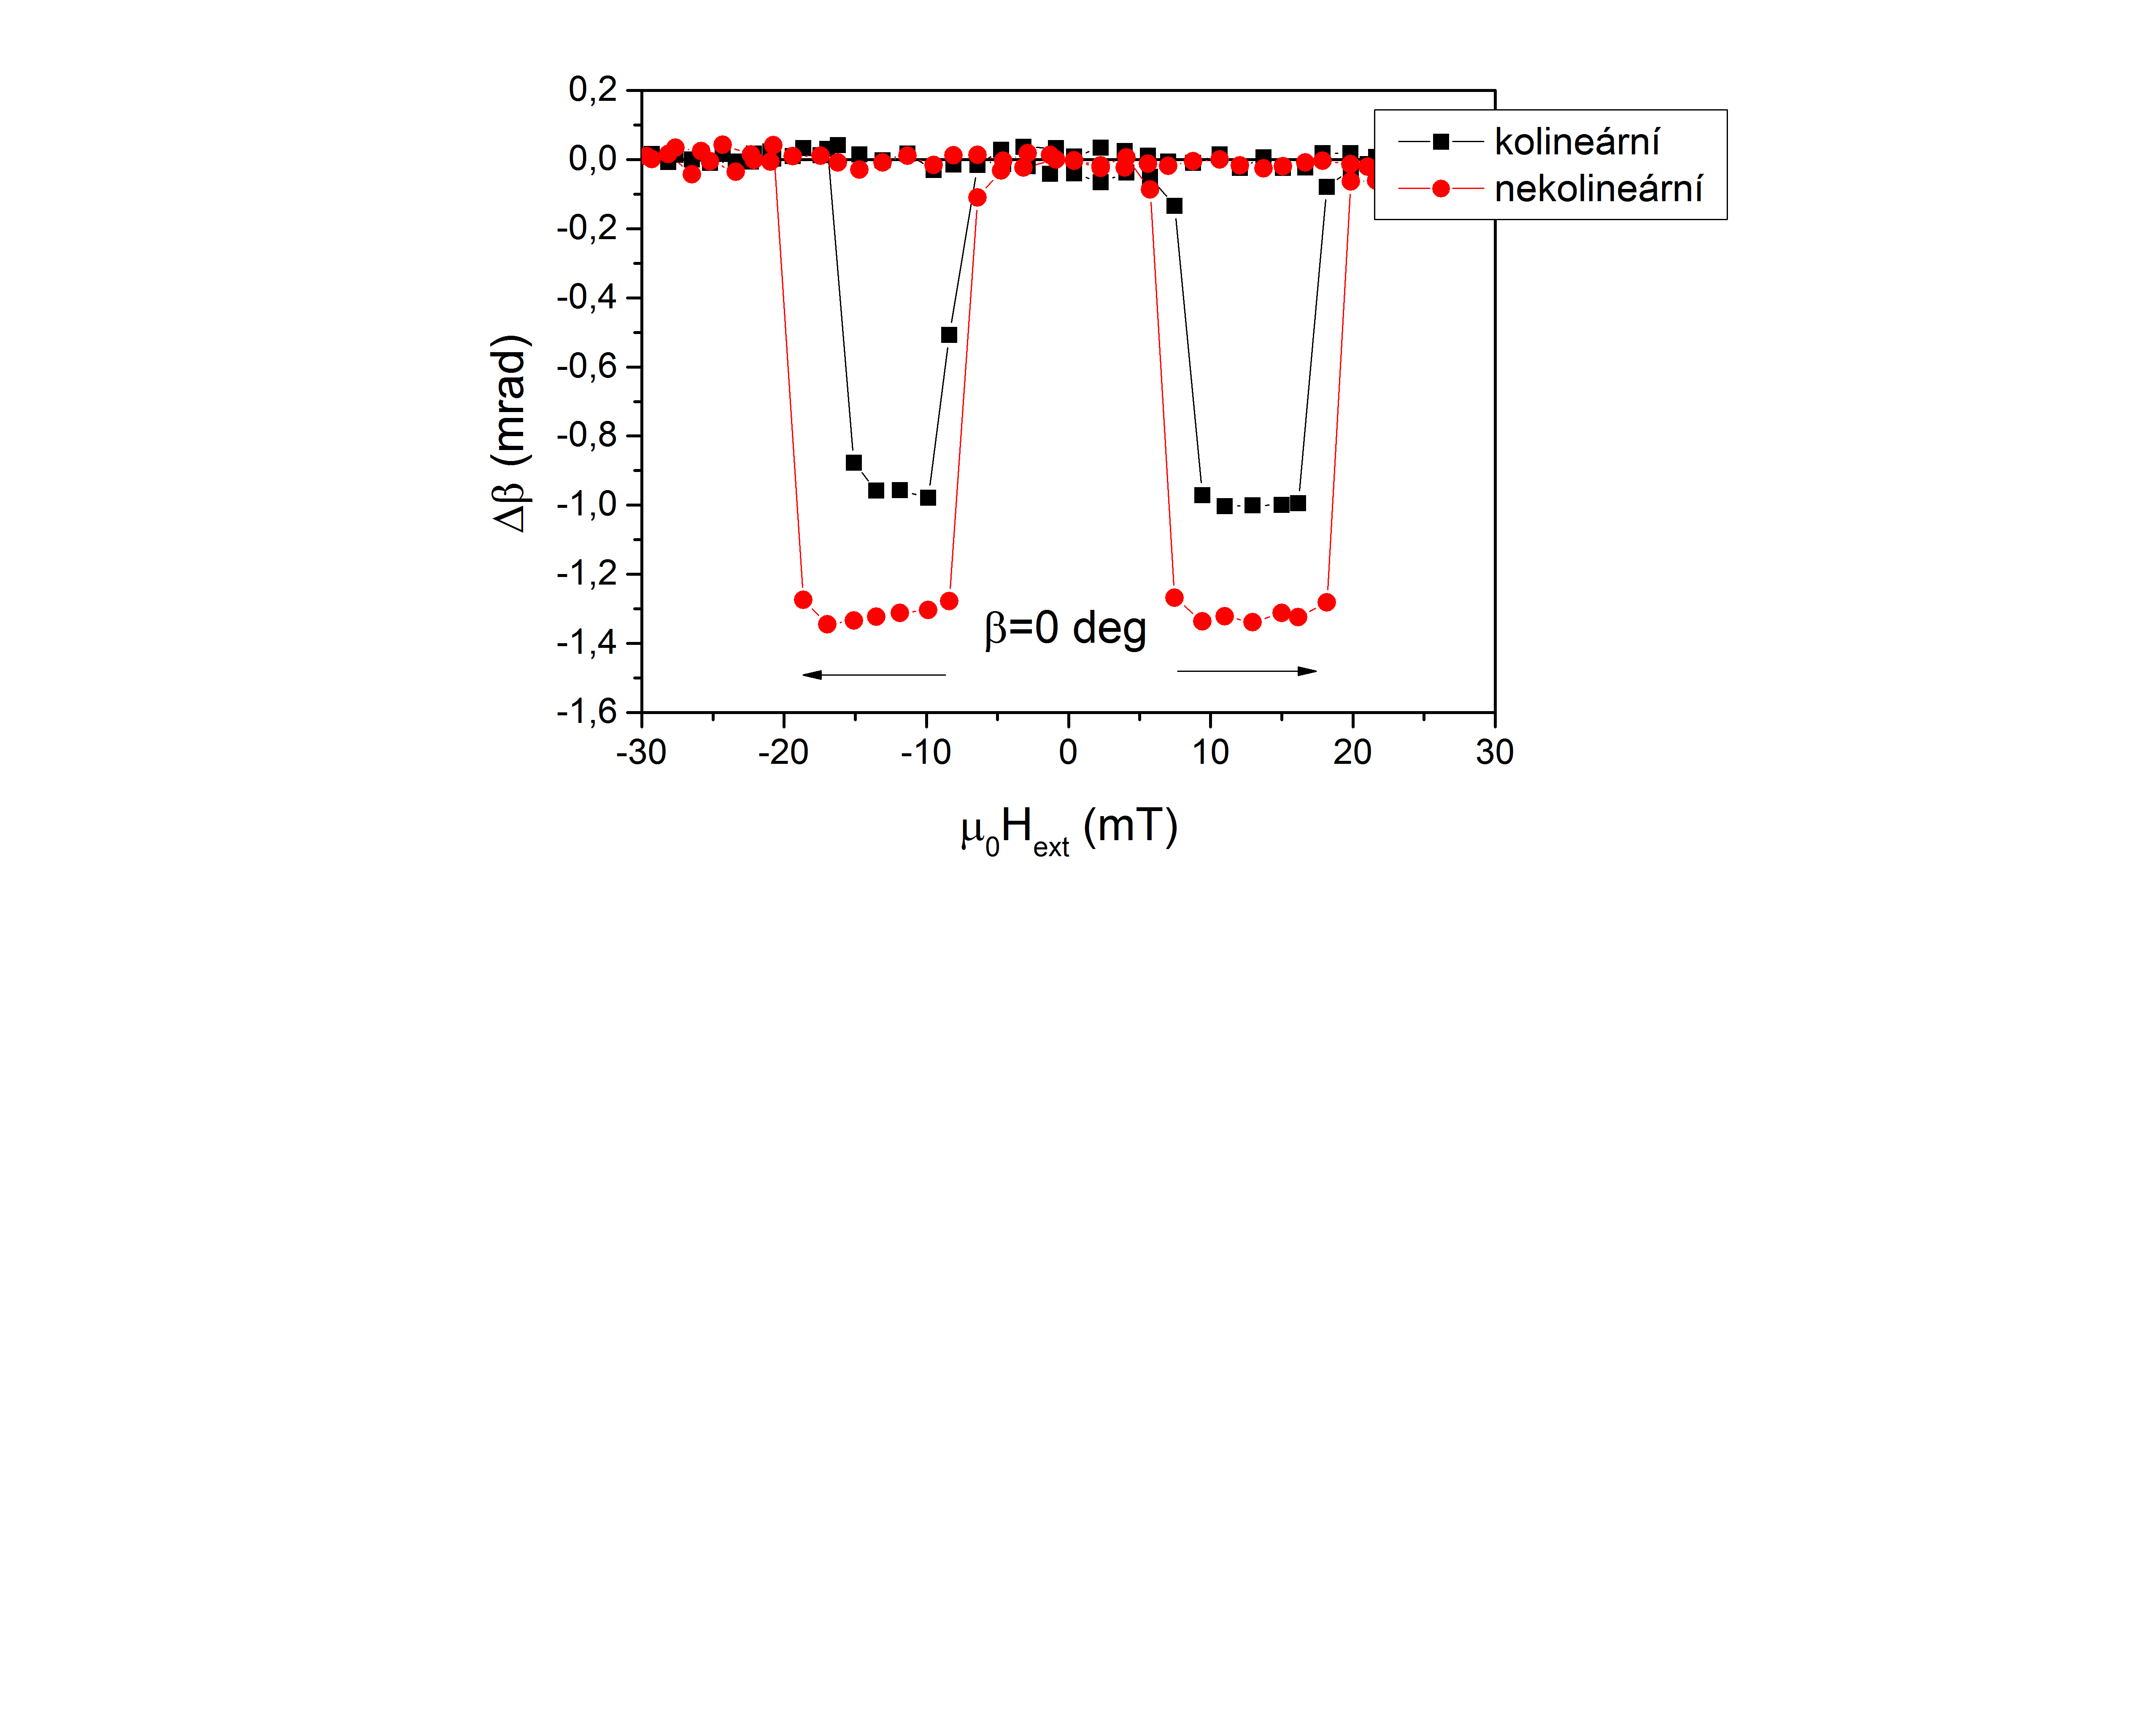
\includegraphics[trim={0 3.43in 0 0}, clip, width=\textwidth]{./png/kolhyst_nekol}}
	\caption{Porovnání Voigtova jevu v kolineární a nekolineární geometrii. Měření v kolineární geometrii pravděpodobně proběhla při vyšší teplotě.}\label{kol_nekol}
\end{figure}


\subsection{Závislost na směru vnějšího pole} \label{kap_smer}

Měřili jsme hysterezní smyčky ve všech směrech pole s krokem \ang{15}. Ovládání elektromagnetu má v současné době implementované a zkalibrované pouze čtyři směry: \ang{0}, \ang{45}, \ang{90}, \ang{135}. Zbývajících směrů jsme dosáhli otočením ramena kryostatu se vzorkem o $+\ang{15}$ a $-\ang{15}$. Zároveň se vzorkem jsme točili i rovinu polarizace, aby byla splněna podmínka $\gamma-\beta=\ang{90}$ a Voigtův jev byl maximální.
Směry $\phH>\ang{165}$ jsme měřili jako \emph{down} opačného směru.

Měření proběhlo při teplotě $T<\SI{15}{\kelvin}$ a intenzita laseru dopadajícího na vzorek byla \SI{1,2}{\milli\watt}.

U hysterezních smyček sledujeme veličiny $\hcj$, $\hcd$ a $A$ (viz obr. \ref{kol_okolo}).
Ve směrech \ang{45}, \ang{60}, \ang{225}, \ang{240} jsme nepozorovali žádný magnetooptický signál, protože magnetizace v průběhu hysterezní smyčky zjevně přeskakuje pouze mezi dvěma protilehlými snadnými osami. To je v souladu s očekávanou polohou prvnní snadné osy v tomto vzorku (viz tabulka \ref{tab_vzorek}), která při zvoleném nalepení (viz obr. \ref{souradna_soustava_vzorek}) odpovídá směru $59(5)^\circ$. Překvapivý je ale fakt, že při položení pole ve směru druhé snadné osy, který by se měla nacházet na poloze $121(5)^\circ$, smyčky pozorujeme.

\begin{figure}[htbp]\centering
\qq{	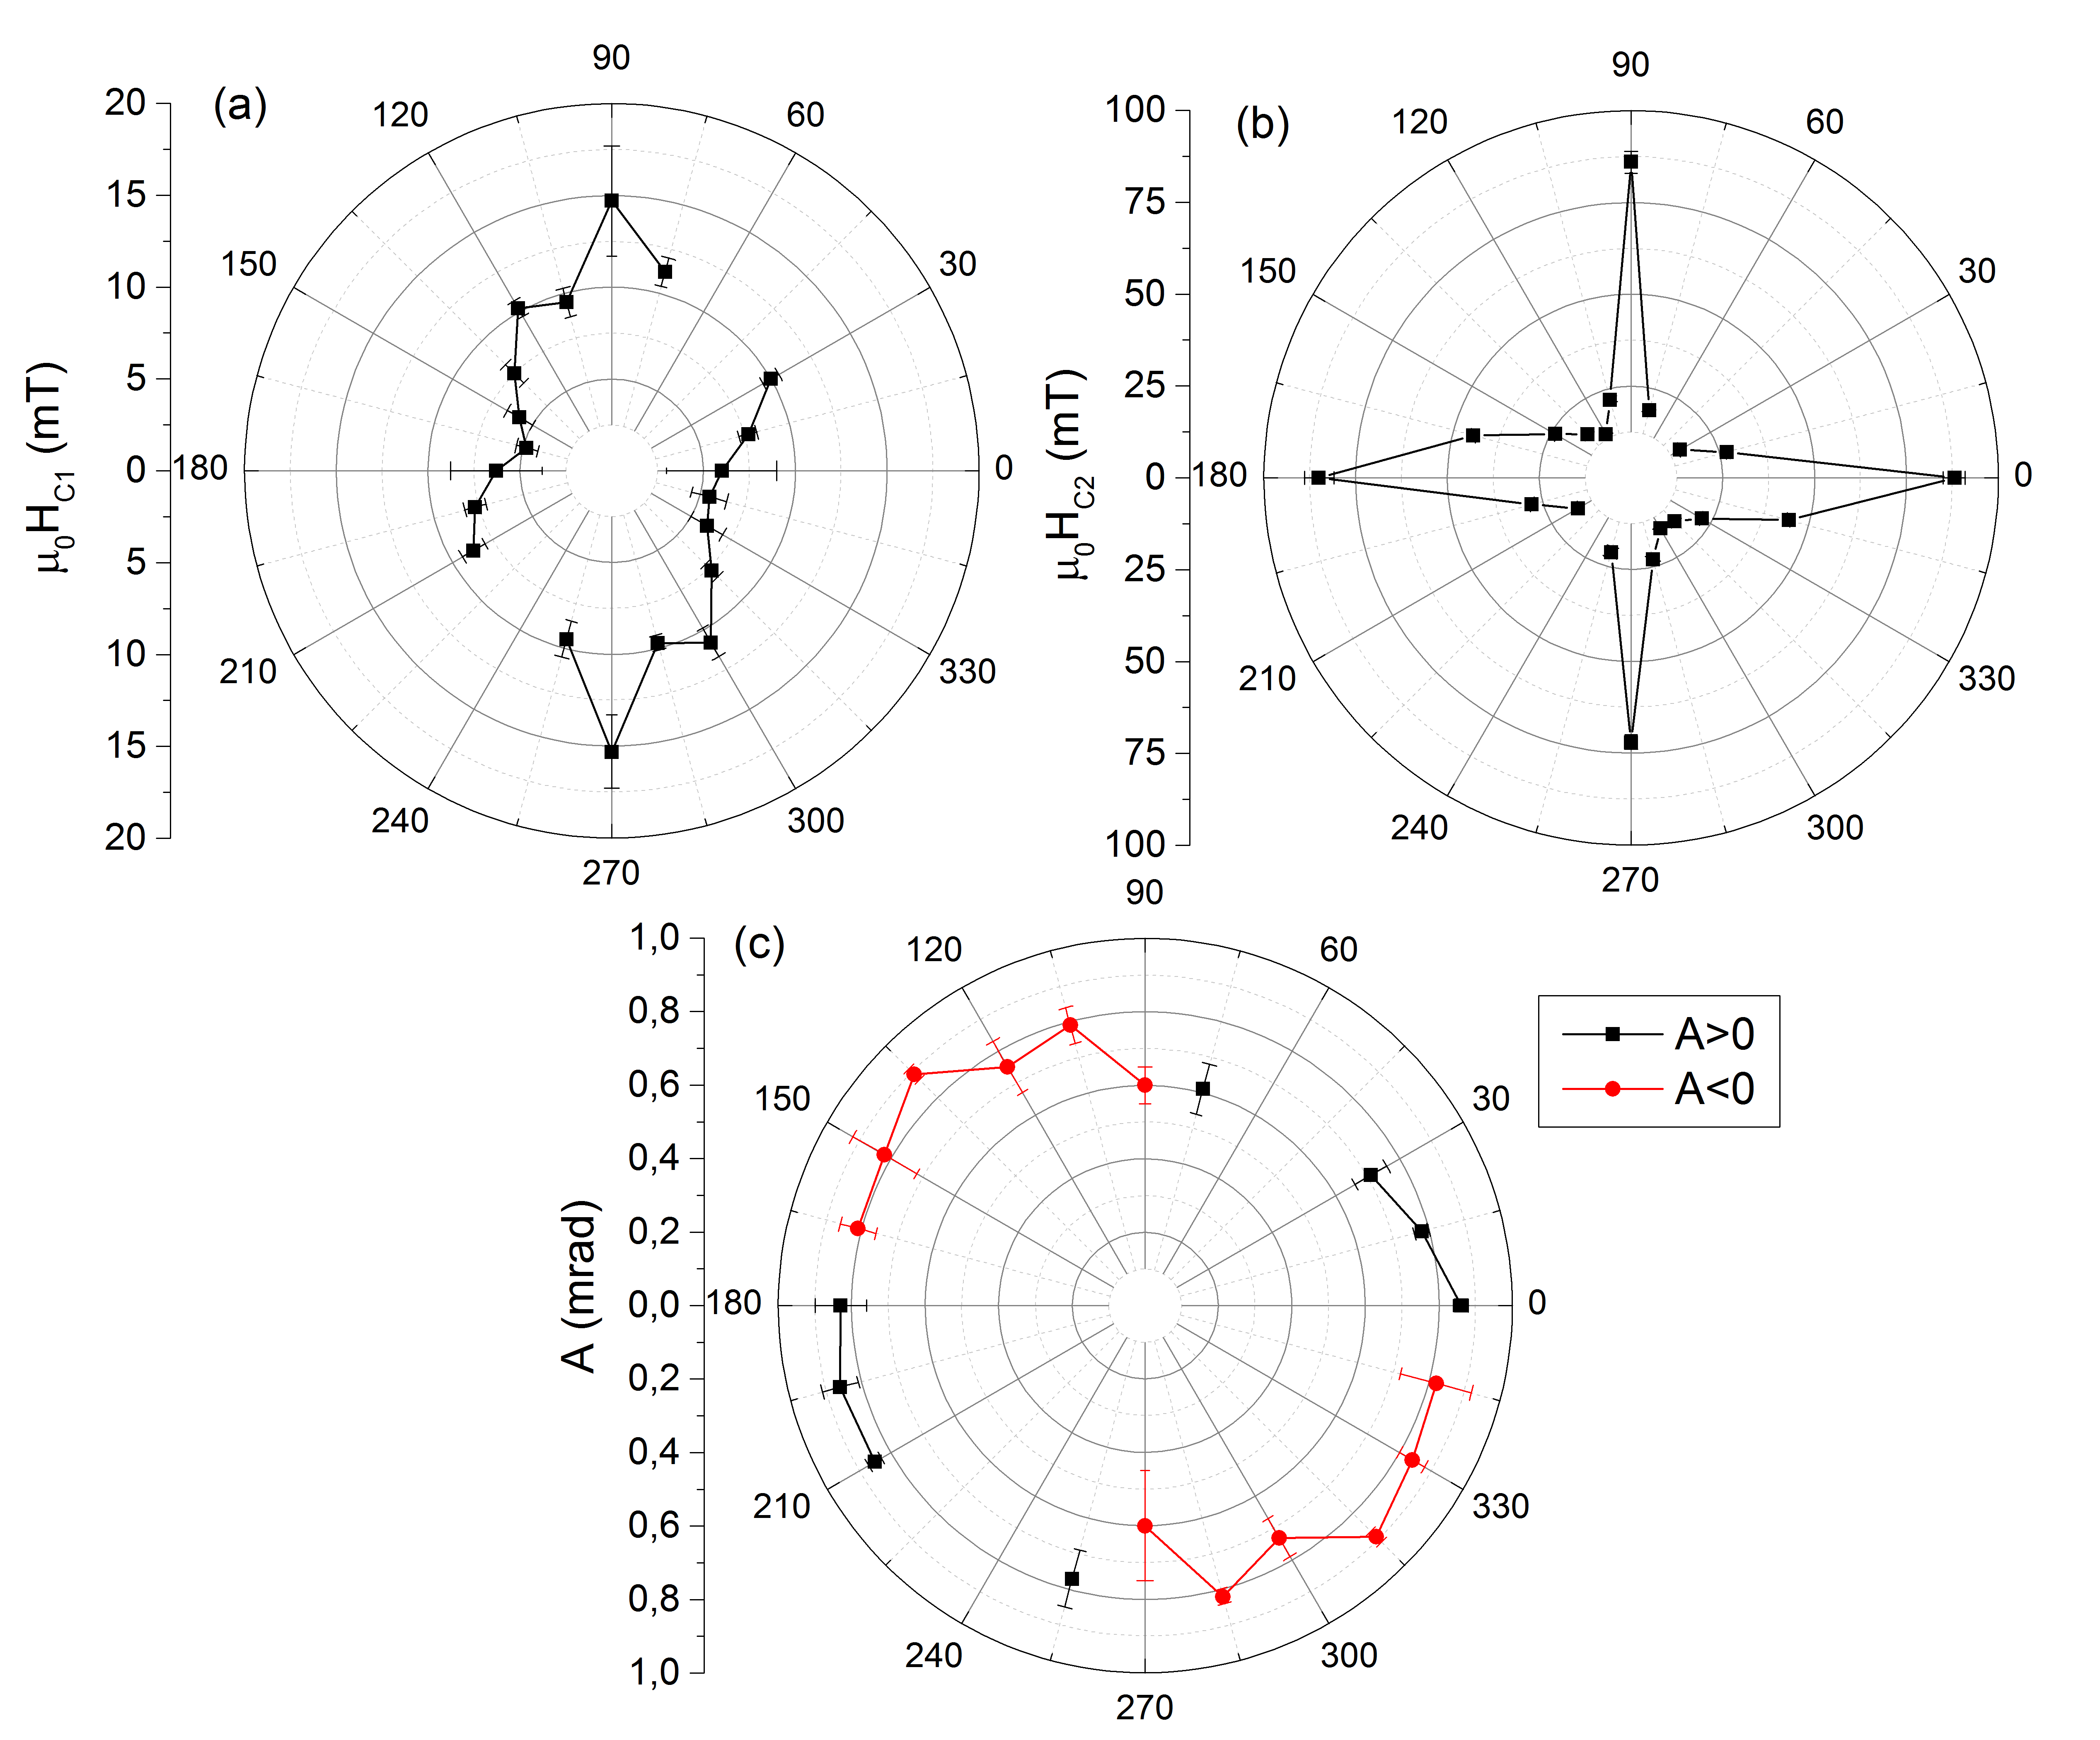
\includegraphics[width=\textwidth]{./png/hystgraf_okolo}}
	\caption{Měření Voigtova jevu v hysterezních smyčkách pro různá $\phH$. (a) Úhlová závislost $\hcj$. (b) Úhlová závislost $\hcd$. (c) Úhlová závislost amplitudy přeskoku $A$. Kladné hodnoty černě, záporné červeně.}\label{kol_okolo}
\end{figure}

Nejzajímavější je graf koercitivních polí $\hcd$, ve kterém jsou jasně patrné významné krystalografické směry [110] a [-110] (porovnejte s \ref{souradna_soustava_vzorek} (b)).



\subsection{Teplotní závislost při vnějším poli ve směru \ang{135}}

Vzorek jsme nejprve zchladili při vypnutém topení ($T=\SI{12(3)}{\kelvin}$). Nastavením teploty na termočlánku jsme vzorek zahřívali s krokem \SI{5}{\kelvin} až do takové teploty, kdy hysterezní smyčky přestaly být patrné. Skutečný rozsah měřených teplot byl 12-\SI{60}{\kelvin}. Intenzita laseru dopadajícího na vzorek byla \SI{2}{\milli\watt}.

Měříme pouze polarizaci $\beta=\ang{0}$, tedy $\gamma-\beta=\ang{90}$.

Teplotní závislost hysterezních smyček je na obr. \ref{kol_vysl_tep_voigt} (a). U hysterezních smyček sledujeme opět veličiny $\hcj$, $\hcd$ a $A$ (viz obr. \ref{kol_vysl_tep_voigt} (b), (c)).


\begin{figure}[htbp]\centering
\qq{	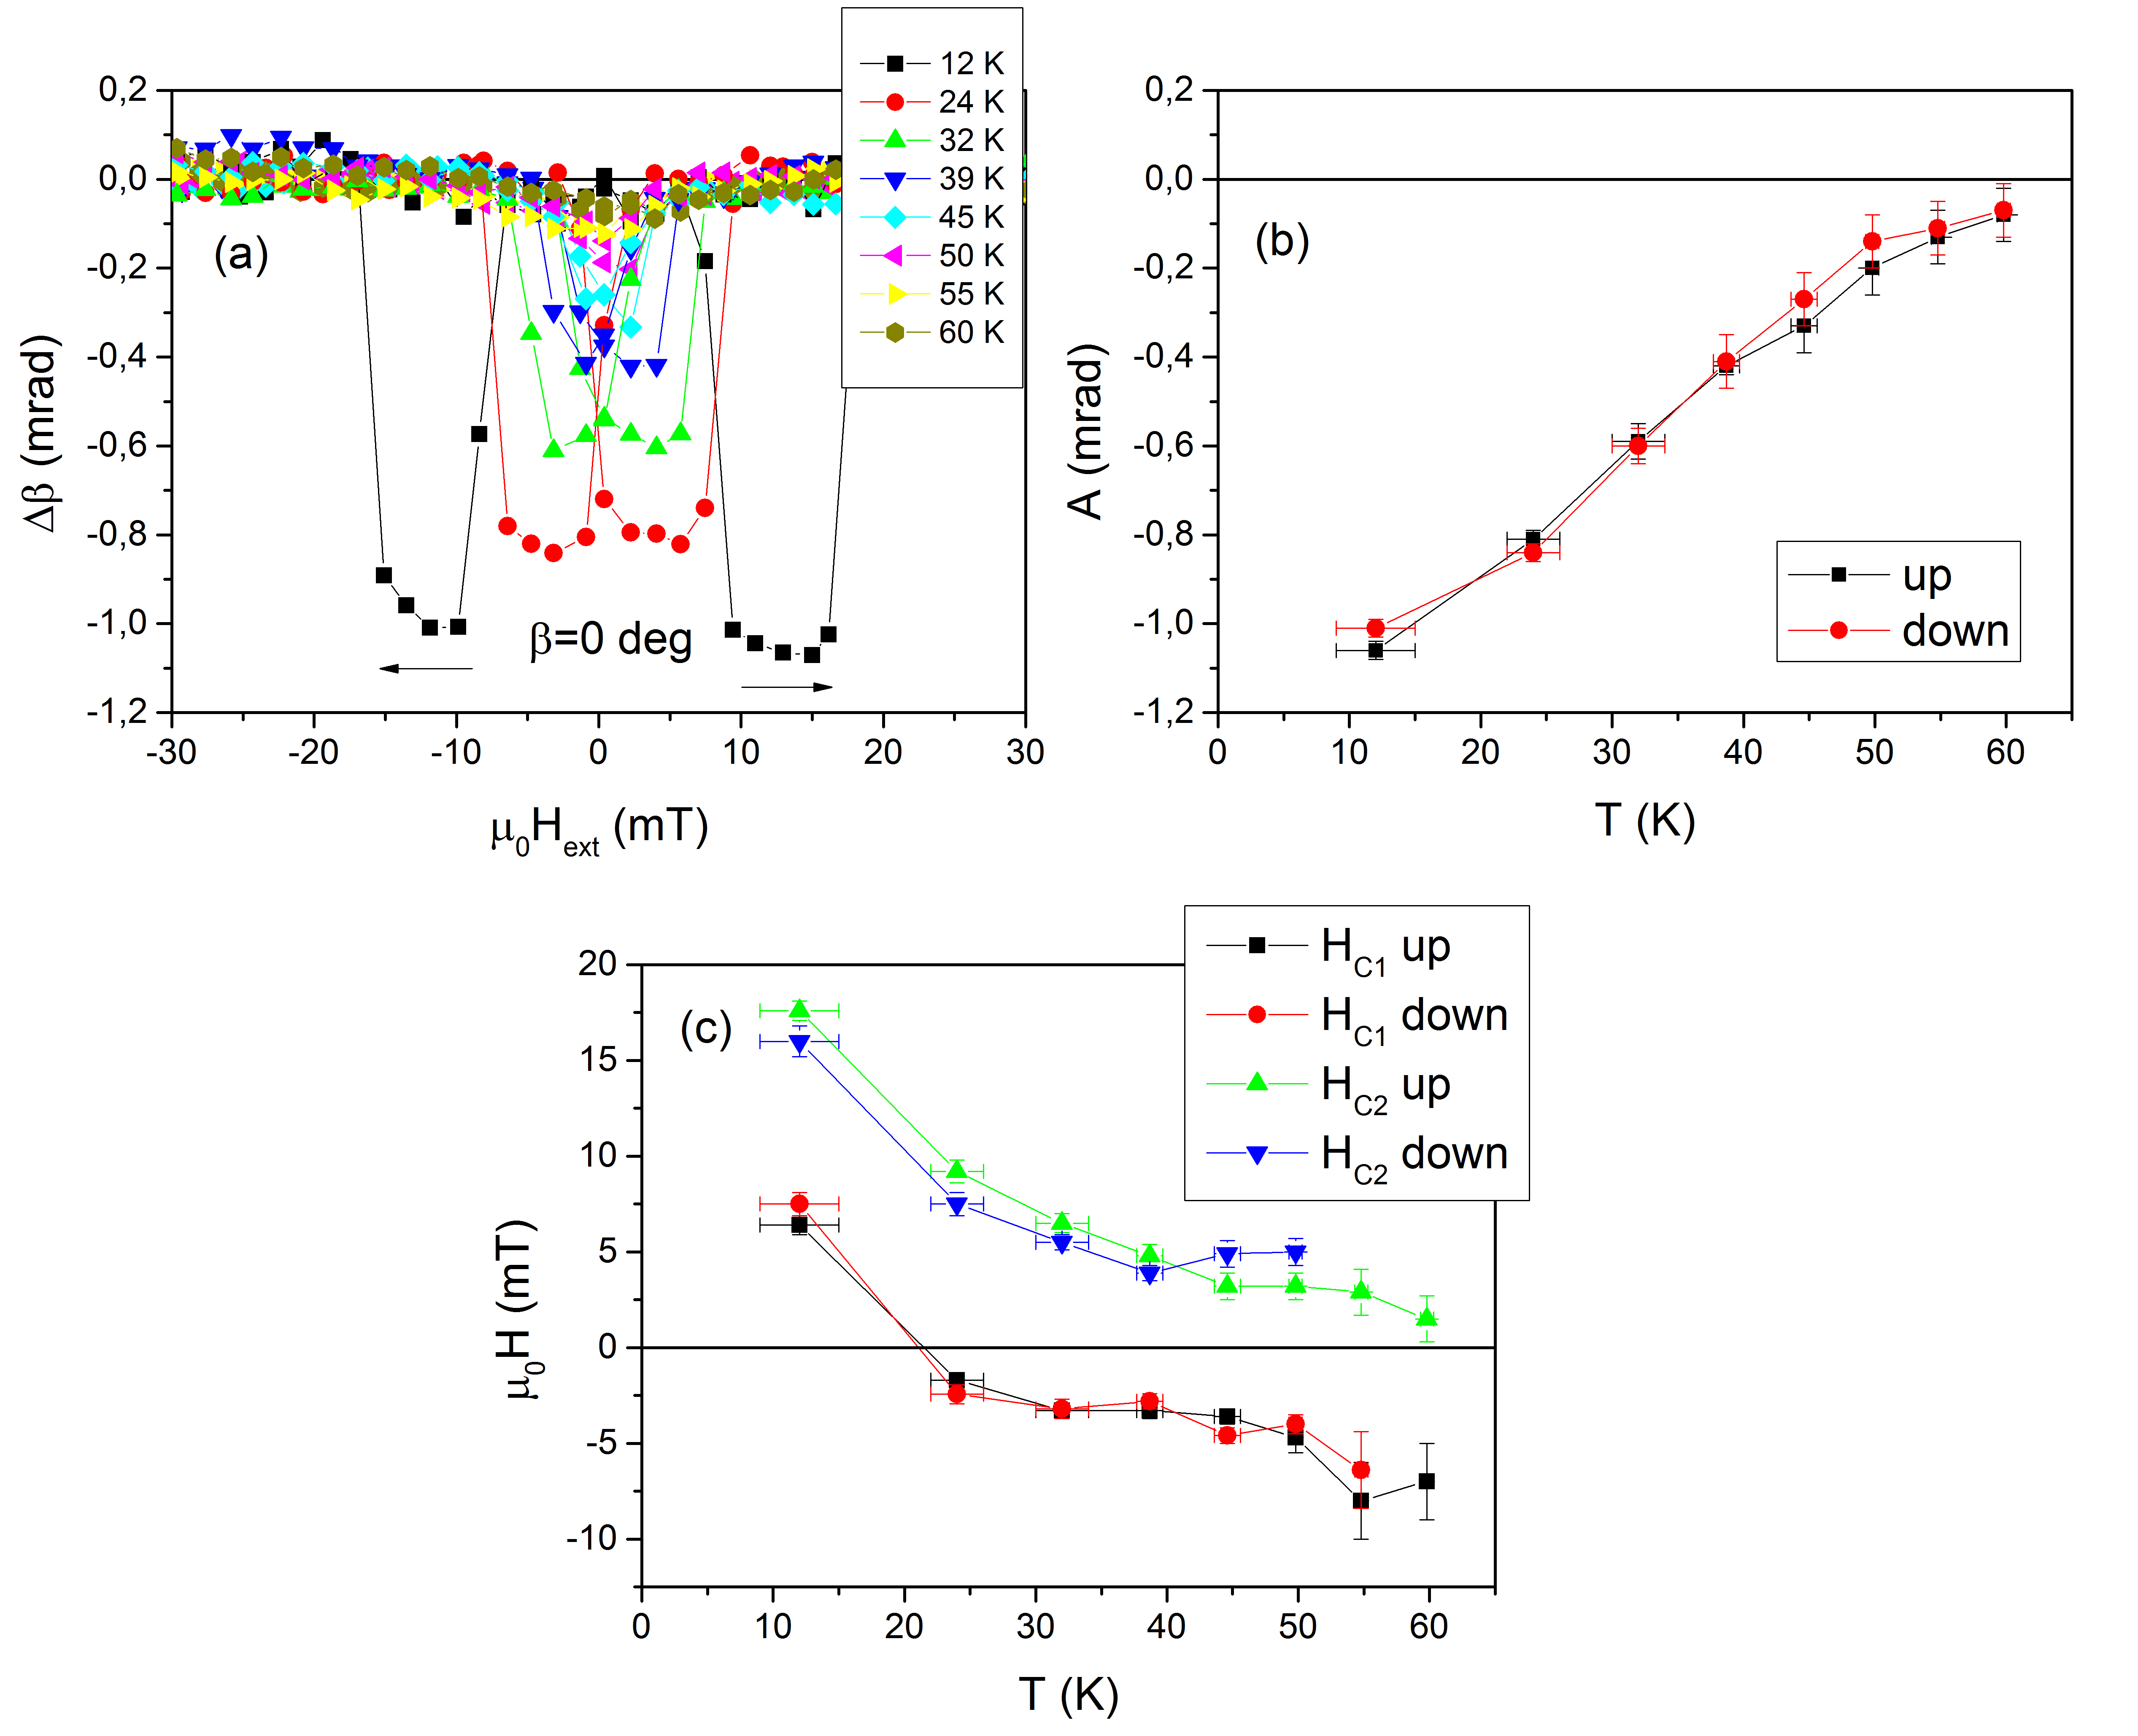
\includegraphics[width=\textwidth]{./png/kolhyst_135tepl}}
	\caption{Měření teplotní závislosti Voigtova jevu v hysterezních smyčkách pro $\phH=\ang{135}$ v kolineární geometrii. (a) Hysterezní smyčky při všech měřených teplotách. (b) Teplotní závislost amplitudy přeskoku $A$. (c) Teplotní závislost koercitivních polí.}\label{kol_vysl_tep_voigt}
\end{figure}
